\documentclass[
%%%%% Styles and Sizes
%10pt,
%11pt,
%12pt,
fancyheadings, % headings with seplines and logo
%
%%%%% Printing, Color and Binding
%a4paper,
%a5paper,
%twoside, % single sided printout
%oneside, % duplex printout (default)
%% binding correction is used to compensate for the paper lost during binding
%% of the document
%BCOR=0.7cm, % binding correction
%nobcorignoretitle, % do not ignore BCOR for title page
%% the following two options only concern the graphics included by the document
%% class
%grayscaletitle, % keep the title in grayscale
%grayscalebody, % keep the rest of the document in grayscale
%
%%%%% expert options: your mileage may vary
%baseclass=..., % special option to use a different document baseclass
]{stsreprt}

\usepackage{algorithm}
\usepackage{algpseudocodex}
\usepackage{amssymb}
\usepackage[english]{babel}
\usepackage{biblatex}
\usepackage{booktabs}
\usepackage{csquotes}
\usepackage{mathtools}
\usepackage{microtype}
\usepackage[binary-units]{siunitx}
% \usepackage[section]{placeins}
\usepackage{subcaption}
\usepackage{tikz}
\usepackage{hyperref}
\usepackage[capitalise, noabbrev]{cleveref}

\addbibresource{refs.bib}

\usetikzlibrary{graphs,graphdrawing}
\usegdlibrary{trees}

% Common Grapple algorithm subroutines
\DeclareMathOperator{\markVisited}{\texttt{mark\_visited}}
\DeclareMathOperator{\qEmpty}{\texttt{queue\_empty}}
\DeclareMathOperator{\qPop}{\texttt{queue\_pop}}
\DeclareMathOperator{\qPush}{\texttt{queue\_push}}
\DeclareMathOperator{\sSuccessor}{\texttt{state\_successor}}
\DeclareMathOperator{\sViolates}{\texttt{state\_violates}}

% Successor generation subroutines
\DeclareMathOperator{\branchFreeTernary}{\texttt{BranchFreeTernary}}

% Bitstate hashing subroutines
\DeclareMathOperator{\makeHash}{\texttt{make\_hash}}

% Inline citation, e.g. "Foobar" by J. Doe [27]
\newcommand{\citeinline}[1]{\citetitle{#1} by \citeauthor*{#1} \cite{#1}}

% Biwise operators
\newcommand{\bitwiseAnd}{\mathbin{\text{\&}}}
\newcommand{\bitwiseOr}{\mathbin{\text{|}}}

% Information for the Titlepage
\author{Leonard Techel}
\title{Low-Connectivity State Space Exploration using Swarm Model Checking on the GPU}
\date{September 27, 2021}
\subject{Bachelor Thesis}
\professor{Prof. Dr. Sibylle Schupp}
\advisor{Sascha Lehmann}

\begin{document}

\frontmatter

\maketitle

\begin{otherlanguage}{ngerman}
    \chapter*{Eidesstattliche Erklärung}

    Ich erkläre hiermit an Eides Statt, dass ich die vorliegende Arbeit selbständig sowie ohne unzulässige Hilfe Dritter und ohne Benutzung anderer als der angegebenen Hilfsmittel angefertigt habe.
    Die aus anderen Quellen direkt oder indirekt übernommenen Daten und Konzepte sind unter Angabe der Quelle gekennzeichnet.
    Die Arbeit wurde in gleicher oder ähnlicher Form noch keiner anderen Prüfungsbehörde vorgelegt.

    \vspace{2.5cm}

    \noindent Hamburg, den 27. September 2021
\end{otherlanguage}

\chapter*{\centering \begin{normalsize}Abstract\end{normalsize}}
\begin{quotation}
    % 1. Motivation / Topic of the research area
    Using small, independent verification tests, model checking large models with billions of states can be parallelized on GPUs.
    % 2. Specific problem
    This approach works great on models with high connectivity.
    However, it fails when a model has only few edges between states or large portions of the state space are hidden behind bottleneck structures.

    % 3. Standard solutions and their limitations
    Past work on the \emph{Grapple} model checker has tried different approaches including depth-limiting and alternating between breadth-first and depth-first search.

    % 4. Outline of the new solution
    The main goal of this thesis is to:
    (1) create a systematic way of classifying a model as \emph{low-connectivity}
    (2) minimize the amount of verification tests needed to maximize the state space coverage of said models.
    To do that, we provide an implementation of the \emph{Grapple} model checker.

    % 5. How the solution was evaluated and what its outcomes are
\end{quotation}

\tableofcontents
\listofalgorithms
\listoffigures
\listoftables

\mainmatter

\chapter{Introduction}

% 1. Motivation / Topic of the research area
Swarm verification is an approach on explicit-state model checking that tackles the state explosion problem by splitting the state space exploration into many small, independent verification tests (VTs), each covering only a subset of the state space.
As VTs are small and independent, they can be parallelized on the GPU, resulting in high-speed model checking that can outperform the execution time of similar CPU-based approaches by multiple degrees.
% 2. Specific Problem
Past work has shown that low-connectivity models with only few edges between states, or large portions of the state space hidden behind bottleneck structures, can cause a swarm model checker to achieve significantly less state space coverage.

% 3. Standard solutions and their limitations

% 4. Outline of the new solution
In this thesis, we provide the following contributions to swarm model checking on the GPU and the exploration of low-connectivity models:

\begin{itemize}
    \item A method for estimating unique states visited with a fixed error in a swarm verification.
          This allows the observation of progress in state space coverage and giving probabilistic guarantees on models with known state space size.
    \item A Grapple search strategy extension called \emph{start overs} that can reach deeper states by continuing the search within a VT multiple times.
          Furthermore, the strategy allows using even smaller hash tables by compensating lost hash table capacity with additional start overs.
    \item A visualization of unvisited and visited states in the frontiers of Grapple's breadth-first search that shows promising characteristics on a set of low-connectivity models.
    \item An in-depth explanation of the Grapple state space exploration loop by breaking it down into subroutines.
    \item An experimental implementation of a Grapple model checker, including a selection of models specifically implemented for on-the-fly verification on the GPU
\end{itemize}

% 5. How the solution was evaluated and what its outcomes are
Comparison with the swarm verification waypoints benchmark has shown that our unique states visited estimation provides reliable results.
We compared the progress in state space coverage of our start over strategy on multiple models, including the waypoints benchmark and the well-known dining philosophers problem.
On those models, our start over strategy has shown a significant increase in state space coverage on a similar number of visited states and VTs in comparison to the default Grapple algorithm.

A notable exception has been the Anderson queue lock mutual exclusion algorithm.
Using our start over strategy, state space coverage has worsened significantly.
Furthermore, the model has shown interesting behavior in the visualization of its BFS frontiers.

% 6. Structure of the thesis
The rest of this thesis is structured as follows:
We start with an overview of related work in \cref{chapter:related-work}.
A brief summary on model checking, swarm verification and the CUDA GPU programming framework is given in \cref{chapter:background}.
The Grapple algorithm's components, swarm diversification techniques, including our start over strategy, and the unique states visited estimation are explained in \cref{chapter:theory}.
Our concrete implementation is presented in \cref{chapter:implementation}.
An extensive series of experiments comparing our implementation with the Grapple paper, and experiments comparing low-connectivity models with the waypoints benchmark model, is conducted in \cref{chapter:evaluation}.
Last but not least, we conclude our results and give an outlook to additional interesting research problems arisen by this thesis in \cref{chapter:conclusion}.

\chapter{Related Work}
\label{chapter:related-work}

\emph{Swarm Verification} was first studied by \citeauthor*{Holzmann2008.Swarm-Verification} as verification method for models with large state spaces on which an exhaustive verification cannot be completed in any reasonable amount of time due to the state explosion problem \cite{Holzmann2008.Swarm-Verification}.
It was first used as an extension to the SPIN model checker.
Techniques for implementing swarm verification were introduced in \cite{Holzmann2011.Swarm-Verification-Techniques}, including a memory-efficient method of marking states as visited called \emph{bit state hashing}, multiple state space diversification techniques, and an evaluation of swarm verification performance on real-world models.

This thesis is based on the Grapple model checking framework \cite{DeFrancisco2020.Grapple}.
They implement an explicit-state \cite{Holzmann2018.Explicit-State-Model-Checking}, on-the-fly, parallel swarm verification model checker on the GPU using the CUDA framework \cite{CUDA-Programming-Guide}.
Our implementation tries to stay as close as possible to theirs, with three noteworthy exceptions:

\begin{itemize}
    \item To simplify the bit state hashing, we calculate bucket and element using bit shifts instead of arithmetic operations, resulting in a smaller hash table as we cannot address the full \SI{48}{\kibi\byte} of shared memory.
    \item To estimate unique states visited, we use a HyperLogLog++ instead of accurate counting using a global hash table.
    \item To go deeper in a state space exploration, we extend the algorithm by a self-contained strategy named \emph{start overs} that is applied directly on-device within the GPU kernel, instead of the scatter-PDS approach used in Grapple where continuation of a search is controlled by the host.
\end{itemize}

A key difference between Grapple and the SPIN swarm verification is the highly constrained hash table size in Grapple, which stores its hash tables in CUDA's \SI{48}{\kibi\byte} of shared memory.
In the SPIN implementation, the hash table size is decided per model, often multiple megabytes in size.
An evaluation of using small hash tables is done on an implementation of swarm verification using FPGAs, from which Grapple also adapts its structure of internal components within VTs \cite{Cho2018}.
A key observation of said evaluation is that in the SPIN implementation, the waypoints benchmark model is explored fastest using \SI{256}{\mega\byte} hash tables, which is considerably larger than in the FPGA and GPU swarms.
Even though its smaller hash tables, both the FPGA and GPU swarm outperform the SPIN swarm in execution time on the waypoints model, underlining the performance benefit of massive parallelization of swarm verification.

Exhaustive multi-core parallel model checking is a research area with numerous approaches, including parallelization of the SPIN model checker \cite{Holzmann2004} and the parallel DiVinE model checker \cite{Barnat2008, Barnat2007}.
Both approaches share using a parallel breadth-first search (BFS) and support verification of liveness properties.
However, the SPIN approach only supports a sub-class of liveness properties that can be reduced into safety properties called \emph{bounded liveness} \cite{Holzmann2012.Paralellizing-SPIN}.
The Grapple framework is re-using the parallel BFS from the SPIN-approach for parallelization within VTs, which we are explaining in-depth in \cref{section:theory:queues} and \cref{section:implementation:queues}.

In \cite{Bartocci2014.GPGPU-Parallel-SPIN}, the authors of the Grapple framework lay its foundations by extending the SPIN model checker to run its parallel BFS state space exploration \cite{Holzmann2012.Paralellizing-SPIN} on the GPU using CUDA.
Most notably, they already use on-the-fly successor generation on the GPU.
For that, they introduce an algorithm that allows successors to be generated without branching through \texttt{if}-/\texttt{else}-/\texttt{switch}-conditions, which we are explaining in-depth in \cref{section:theory:model-definition} and \cref{section:implementation:successor-generation}.
The leading differences to the Grapple framework are that they perform an exhaustive verification and that synchronization of threads is done using a custom \emph{fast-barrier synchronization} instead of using native CUDA \texttt{\_\_syncthreads()}.

Another approach to model checking on the GPU is performed by DiVinE-CUDA \cite{Barnat2009.DiVinE-CUDA}.
Their work is focussed on finding accepting cycles, and thus verification of liveness properties, by reformulating the maximal accepting predecessors (MAP) algorithm to be conducted as matrix-vector multiplication on the GPU \cite{Barnat2009}.
Even though the approach supports on-the-fly verification using similar operations for successor generation and violation checking as the Grapple framework, it cannot simply be added to a swarm verification.
In swarm verification, no explicit state graph is built up during verification, or in other words, no explicit history of already visited states is kept.
This introduces a severe difficulty on verifying whole paths for liveness properties.

% TODO GPUexplore \cite{Wijs2014, Wijs2016}

Probabilistic cardinality estimation is an extensively covered research area due to its wide range of applications in internet-based applications.
A comparison of available algorithms can be found in \cite{Metwally2008}.
We chose to use the HyperLogLog++ (HLL) algorithm, which improves the HyperLogLog algorithm \cite{Flajolet2007.HyperLogLog} for very large and very small cardinalities, and allows counting beyond a billion, which is necessary to, for example, count unique states visited of the waypoints model.
HLL is a distributed, highly memory-efficient probabilistic cardinality estimator with a fixed error \cite{Heule2013.HyperLogLog++}.
It is especially well-suited for counting unique states visited in swarm verification for multiple reasons:
Most importantly, each HLL takes up only a few kilobytes to count into the billions, meaning that it can be stored in CUDA shared memory.
HLLs can be merged, so independence of VTs is preserved.
Due to \texttt{add} and \texttt{estimate} operations being separate from each other, we can use only the low-complexity \texttt{add} operation on the GPU and defer the estimation to the host, so no significant computational overhead is added to the state space exploration.
Having a fixed error, it creates the possibility of giving probabilistic guarantees on the state space coverage of a swarm verification.

Looking beyond model checking, \emph{graph partitioning} is an intuitively related problem to swarm verification.
In graph partitioning, a graph is cut into mutual exclusive groups, so, for example, distributed algorithms can be run on them.
An interesting approach in terms of on-the-fly verification are the streaming graph partitioning algorithms, which receive edges or vertices of a graph in a random order as inputs and produce partitions on them using heuristics \cite{Stanton2012}.
A main difference to diversification in swarm verification is that states are distributed onto their partitions as they arrive, which, in a naive implementation, would require the search for violations to be conducted as separate step after partitioning.

\chapter{Background}
\label{chapter:background}

This chapter gives a brief summary on the main topics that this thesis is based on.
First, we define the scope of model checking that we are looking at in \cref{section:background:model-checking}.
We continue with an overview of Swarm Verification on the GPU and the specific problem that we are going to investigate, low-connectivity state space exploration, in \cref{section:background:parallelized-model-checking}.
Last but not least, we give an introduction to the CUDA GPU programming framework in \cref{section:background:cuda}.

\section{Model Checking}
\label{section:background:model-checking}

% What is a model checker?
% TODO Why do we search for counterexamples? The answer may fit better to the properties paragraph.
% TODO Why can it be divided into three main problems and why the specific methods stated here?
Model checking is a formal verification method that checks whether a state machine satisfies a specification.
For example, the state machine of an elevator may be verified to meet the safety property of not opening the doors between floors.
To do so, a \emph{model checker} searches the state space for counterexamples, also called violations.
When a violation is found, the path of state transitions that leads to the violation is reported back.

Model checking can be divided into three main problems:
Description of models through state machines, definition of the specification through temporal logic, and algorithms that verify whether a state machine models a specification.

%% What is an explicit-state model checker?
There are two main branches of model checking:
Explicit-State Model Checking and Symbolic Model Checking.
Explicit-State Model Checking can only verify finite state machines.
In particular, the model has to have finite states, each state needs to be representable by a finite-size tuple containing its atomic propositions, and the model changes state through execution of state transitions.
To overcome these limitations and verify potentially infinite-size state machines or systems of unknown structure, Symbolic Model Checking uses the abstraction of \emph{symbols}, each representing a set of states and transitions.
Within this thesis, we are only considering explicit-state model checking.

%% What do we want to find out with a model checker? safety, reachability, liveness, ...
% TODO Connection to temporal logic? Eventually we can skip that here.
Each state in a model is labelled with atomic propositions that hold true while the state is active.
An example for such propositions are the current values of variables in a program at a given state.
In a specification, different types of properties can then be expressed onto these propositions.
Three common properties are reachability, safety and liveness:
Reachability means that an atomic proposition holds true at some state in the future.
Safety means that an atomic proposition holds true at all states in the future.
Liveness means that an atomic proposition holds true infinitely often in the future, meaning that it does not happen that the atomic proposition never holds true.
Within this thesis, we are only considering reachability and safety properties.

%% Why is model checking so time consuming?
% TODO Introduce processes in the explicit-state model checking section
% TODO Be more precise about *what* grows exponentially and *why* this is a problem
A challenge all model checking algorithms have to face is the \emph{state explosion problem}.
In an asynchronous model of $n$ processes, each consisting of $m$ states, the number of states grows exponentially by the number of processes, namely $m^n$.
This means that even for small models, it is often not possible to fit all reachable states of the system into a computer's memory.
Therefore, every model checking algorithm needs to reduce the state space in some sense.
However, even then, a non-parallel algorithm may need a lot of physical time for exhaustive verification of the state space.
In exhaustive verification, all states are visited and checked for a violation.
\cite{Clarke2018.Introduction-to-Model-Checking,Holzmann2018.Explicit-State-Model-Checking}

\section{Parallelized Model Checking}
\label{section:background:parallelized-model-checking}

% How can model checking be speed up using parallelization?
% TODO Do we need the algorithm summary?
% TODO If yes, why leave the reader with "we are going to tell later"?
The basic operation in an explicit-state model checker is a state space exploration loop, as defined in \cref{alg:fundamental-state-space-exploration}.
Model checking can be speed up by parallelizing the state space exploration, for example using a parallel breadth-first search (BFS) \cite{Holzmann2012.Paralellizing-SPIN}.

%% What challenge is solved by Swarm Verification?
A major challenge in parallelized BFS is the communication overhead between threads:
Shared memory does not allow to easily split the work onto a cluster of heterogeneous processors or the massively parallel architecture of a GPU on which thousands of threads can exist simultaneously.

\begin{algorithm}
    \caption{Fundamental State Space Exploration Loop}
    \label{alg:fundamental-state-space-exploration}
    \begin{algorithmic}
        \While{there are unvisited states}
        \State mark state as visited
        \If{state violates spec}
        \State report path to state
        \EndIf
        \EndWhile
    \end{algorithmic}
\end{algorithm}

\subsection{Swarm Verification}
\label{section:background:swarm-verification}

%% How does Swarm Verification work?
%% How does Swarm Verification differ from other approaches?
% TODO what is state space exploration?
Swarm Verification is a new approach on parallelized model checking \cite{Holzmann2008.Swarm-Verification}.
It solves the challenge of parallelizing state-space search by splitting the state space exploration into many small, independent, memory-limited tasks called \emph{Verification Tests} (VTs).
Each VT only covers a small subset of the total state space and, using \emph{diversification techniques}, uses a different search path.
By executing all VTs and collecting their results, we still achieve nearly full state space coverage.

% The trick is that we do not care about exhaustive, 100\% state space coverage:

As VTs are independent of each other, we can easily execute them on heterogeneous computers.
Even further, as VTs are also memory-limited, we can massively parallelize them on devices with very limited resources like GPUs.

%% What is diversification and which diversification techniques exist?
Multiple diversification techniques can be applied, e.g. randomizing the order of nondeterministic choice on states with multiple outgoing transitions or reversing the search order.
The fundamental diversification technique is state pruning using hash collisions:
During state exploration, states get marked as visited in a limited-size hash table.
By using a different hash function for each VT, the state space gets automatically pruned through hash collisions.
The process is illustrated in \cref{fig:hash-collision-state-pruning}, that shows an example state graph on which BFS is performed by two VTs.
On the left side, state B and C cause a hash collision, resulting in the subgraph originating in state C being removed.
On the right side, state E and F cause a hash collision, resulting in the subgraph originating in state F being removed.
Each state exploration on its own does not cover the whole state space, however, by combining the results from both searches, all states are covered again.

% TODO How to cite this? It is taken from the Grapple paper :)
\begin{figure}
    \begin{subfigure}[b]{.5\textwidth}
        \centering\resizebox{.8\textwidth}{!}{
            \begin{tikzpicture}[nodes={draw, circle}]
                \graph [tree layout, missing nodes get space] {
                    A [fill=lightgray];
                    B [fill=lightgray];
                    D [fill=lightgray];
                    E [fill=lightgray];
                    F [fill=lightgray];
                    I [fill=lightgray];
                    J [fill=lightgray];

                    A -- B [second];
                    A -- C;
                    A -- D;

                    B -- E;
                    B -- F;

                    C -- F;
                    C -- G;
                    C -- H;

                    D -- I;

                    F -- J;

                    H -- K;
                    H -- L;
                };
            \end{tikzpicture}
        }
        \subcaption*{Collision: \{B, C\}}
    \end{subfigure}
    \begin{subfigure}[b]{.5\textwidth}
        \centering\resizebox{.8\textwidth}{!}{
            \begin{tikzpicture}[nodes={draw, circle}]
                \graph [tree layout, missing nodes get space] {
                    A [fill=lightgray];
                    B [fill=lightgray];
                    C [fill=lightgray];
                    D [fill=lightgray];
                    E [fill=lightgray];
                    G [fill=lightgray];
                    H [fill=lightgray];
                    I [fill=lightgray];
                    K [fill=lightgray];
                    L [fill=lightgray];

                    A -- B;
                    A -- C;
                    A -- D;

                    B -- E;
                    B -- F;

                    C -- F;
                    C -- G;
                    C -- H;

                    D -- I;

                    F -- J;

                    H -- K;
                    H -- L;
                };
            \end{tikzpicture}
        }
        \subcaption*{Collision: \{E, F\}}
    \end{subfigure}
    \caption{State pruning using hash collisions \cite{DeFrancisco2020.Grapple}}
    \label{fig:hash-collision-state-pruning}
\end{figure}

\subsection{Grapple Framework}

% What is Grapple?
The paper \citeinline{DeFrancisco2020.Grapple} which this thesis is based on contributes the \emph{Grapple} framework for parallel swarm verification on the GPU using CUDA.
In their implementation of Swarm Verification, each VT's state space exploration runs in a parallel BFS, using CUDA's built-in synchronization primitives to coordinate threads.

%% Which variations of the algorithm exist?
%% How does the Grapple algorithm work?
%% How can the Grapple algorithm and its in- and outputs be formally defined?

\subsection {Low-Connectivity Models}

% What are Low-Connectivity models?
A key observation of \cite{DeFrancisco2020.Grapple} is that their algorithm's state space coverage in relation to the number of executed VTs slows down on models with \emph{low connectivity}.
A model has \emph{low connectivity} if at least one of the following properties is satisfied:

\begin{itemize}
    \item \textbf{Generally Linear}: The average number of edges per state is close to two: One inbound, one outbound
    \item \textbf{Bottleneck Structures}: A single state or group of states other than the initial state that needs to be passed to reach most of the state space
\end{itemize}

See \cref{fig:lc-ex} for examples of these properties.

%% How can a model be classified as Low-Connectivity? (technically vs. theoretically ?)
%% Why is the Grapple search algorithm so slow on Low-Connectivity models?

\begin{figure}
    \begin{subfigure}[b]{.5\textwidth}
        \centering
        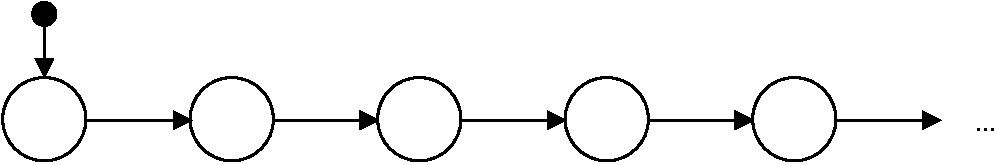
\includegraphics[width=\textwidth]{figures/lc-ex-generally-linear}
        \subcaption{Example of a generally linear graph}
        \label{fig:lc-ex-generally-linear}
    \end{subfigure}
    \begin{subfigure}[b]{.5\textwidth}
        \centering
        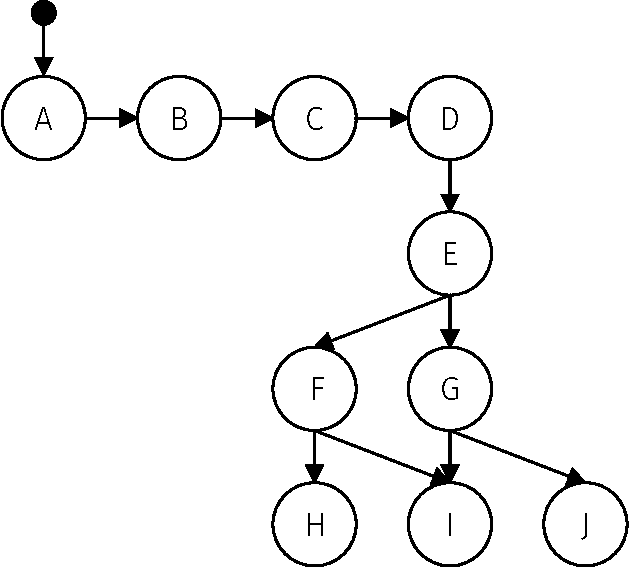
\includegraphics[width=.9\textwidth]{figures/lc-ex-bottleneck}
        \subcaption{Example of a bottleneck structure}
        \label{fig:lc-ex-bottleneck}
    \end{subfigure}
    \caption{Examples of low-connectivity properties}
    \label{fig:lc-ex}
\end{figure}

\section{CUDA}
\label{section:background:cuda}

% How can many small tasks be executed in parallel? What is CUDA?
%% What challenge does CUDA solve?
CUDA is NVIDIA's proprietary GPU programming framework that provides automatic massive scalability \cite{CUDA-Programming-Guide}.

%% What is the abstraction model of CUDA?
The CUDA model defines a three-level abstraction.
At the lowest level, a program function called \emph{kernel} is defined using C/C++.
The kernel is executed by defining the amount of \emph{threads} and \emph{blocks} that run in a \emph{grid}:
Each grid contains multiple blocks.
Each block contains multiple threads.
Each thread in a block executes the kernel function using the single instruction, multiple thread (SIMT) execution model.
Thus, each thread should work on an independent piece of memory.
Only threads within a block can cooperate, for example using shared memory or synchronization barriers.
Internally, the GPU, also called \emph{device}, maps the blocks of threads onto its \emph{streaming multiprocessors}.
By doing so, tens of thousands of threads can be executed in parallel.
The architecture allows scaling even further onto multiple GPUs.

Furthermore, CUDA defines multiple memory levels, each with different size and access speed.
% CUDA Toolkit v11.4.1, Programming Guide, Table 15

\begin{itemize}
    \item \emph{Registers} are used for thread-local variables.
          There can be at max 255 registers à 32 bit per thread.

          % \item \emph{Local memory}

    \item \emph{Shared memory} can only be accessed by the threads of the block in which it got allocated.
          As it is on-chip, it is faster than global memory.
          By default, there is \SI{48}{\kibi\byte} of shared memory.

    \item \emph{Constant memory} is part of the device memory, with the constant cache in front of it.
          Cache hits are served at higher speed than just using global memory.
          There is \SI{64}{\kibi\byte} of constant memory.

          % \item \emph{Texture cache}

    \item \emph{Global memory} is the largest memory with usually multiple gigabytes of size.
          It is placed in device memory and thus also the slowest.
\end{itemize}

%% Why are GPUs so interesting for swarm verification / model checking?
CUDA requires the problem to be solved by a program to be split into many small sub-problems.
This is a good fit with Swarm Verification, which turns the model checking problem into many small, independent VTs.

% - Challenge: Where to parallelize?

% TODO Graphic of the CUDA architecture
% TODO Example CUDA kernel, as in the intermediate presentation

\chapter{Theory}
\label{chapter:theory}

This chapter gives a detailed explanation of the algorithms used by our model checker.
It starts with a formal definition of transition systems in \cref{section:theory:model-definition}.
We continue with an in-depth description of the Grapple framework's state space exploration loop and its components in \cref{section:theory:grapple-model-checker}
Following that, we present a list of known state space diversification techniques and our \emph{start over} extension to the Grapple algorithm in \cref{section:theory:state-space-diversification}.
Then, an explanation of the waypoints model commonly used to benchmark swarm model checkers follows in \cref{section:theory:waypoints-model}.
We finish the chapter with a solution to the problem of counting the number of unique states visited in Swarm Verification in \cref{section:theory:counting-unique-states-visited}.

% TODO what about the theory behind low-conn models ?

\section{Model Definition}
\label{section:theory:model-definition}

As explained in \cref{section:background:model-checking}, a model consists of a transition system and a specification that the transition system is verified for.
%% How are Models defined?
To formally define a model's transition system, we are using a \emph{Kripke Structure} \[M = \left(S; S_0; R; L \right)\] where $S$ is a finite set of states, $S_0 \in S$ is a finite set of initial states $S_0 \subseteq S$, $R \subseteq S \times S$ is a left-total transition relation and $L : S \mapsto 2^{AP}$ is a labelling function that assigns each state its atomic propositions.

%% How are properties defined? (temporal logic)
To define verification properties, Kripke structures are traditionally used in conjunction with temporal logic.
In this thesis, we focus on the state space exploration part of model checking.
Verification of states is thus abstracted away into the $\sViolates$ subroutine and not further covered.
By calling the subroutine on every visited state, we can still be sure that all violations in the covered state space are found, as long as the subroutine is correct.

\section{Grapple Model Checker}
\label{section:theory:grapple-model-checker}

% How can the verification tests be run on GPUs using CUDA?
In Grapple, each VT executes an internally parallel state space exploration.
We call it \emph{internally parallel} to differentiate between the parallelism \emph{within} a VT and the parallelism \emph{between} multiple VTs.
Each thread in a VT executes \cref{alg:grapple-state-space-exploration}, which is a modified version of the Grapple state space exploration loop \cite[Algorithm 1]{DeFrancisco2020.Grapple} using subroutines.
We use subroutines to separately reason about queue operations, successor generation and marking states as visited.
We are going to call this algorithm the \emph{Grapple algorithm}.
The Grapple algorithm is based on \citeauthor*{Holzmann2012.Paralellizing-SPIN}'s parallel BFS \cite{Holzmann2012.Paralellizing-SPIN}.

The following explanation of the algorithm is split into four parts:
We start with a classification of Grapple's state generation strategy and its constraints imposed onto models in \cref{section:theory:model-definition-state-generation}.
Based on that, we explain Grapple's parallel breadth-first search and define the corresponding queue operations in \cref{section:theory:queues}.
Having the successor generation and parallel breadth-first search ready, we can finally define the single operation of the hash table in \cref{section:theory:hash-table}.
Last but not least, we take a look at properties of the algorithm, including termination, in \cref{section:theory:grapple-properties}.

\subsection{Model Definition and State Generation}
\label{section:theory:model-definition-state-generation}

% What constraints does the

%% What is the difference between on-the-fly and a priori state generation?
State generation strategies of model checkers can be divided into \emph{a priori} and \emph{on-the-fly} generation.
In a priori generation, the state space graph is completely known before running the verification algorithm, for example as an adjacency matrix.
In on-the-fly generation, the successors of each state are created on the fly during verification.
Grapple uses on-the-fly generation on the GPU.

As defined in \cref{section:theory:model-definition}, the transition relation of a model is left-total, meaning that for each state, there is at least one successor.
We can define a function returning the successor set of a single state by
\begin{align*}
    \operatorname{succ} : S & \to S' \subseteq S                          \\
    s                       & \mapsto \left\{ s' : (s, s') \in R \right\}
\end{align*}
This function allows each state to have a successor set with different cardinality.
In Grapple, the successor set of a state is called its \emph{nondeterministic choices} (NDCs), highlighting the fact that any of them is a valid continuation of a path through the model's transition system.
% TODO define pathes
To leverage the performance benefit of the GPU's SIMT execution model, Grapple's successor generation has to be branch-free, so each thread can follow the same execution path.
To achieve that, the Grapple algorithm constraints the models it can verify to those with an equal number of NDCs for all states, i.e.\[ \forall s_1, s_2 \in S : |\operatorname{succ}(s_1)| = |\operatorname{succ}(s_2)| \]

Furthermore, Grapple can verify multi-process models.
Following that, we can extend the definition of our transition system by the number of processes and NDCs: \[M_{\text{Grapple}} = \left(S; S_0; R; L; P; \mathit{NDC}\right)\]

%% Which operations does the model have?
The algorithm then uses two subroutines for successor generation and violation checking:
\begin{align*}
    \sSuccessor & : S \times \mathit{NDC} \times \mathit{P}  \to S \\
    \sViolates  & : S \to \left\{0, 1\right\}
\end{align*}
The subroutine $\sSuccessor$ on-the-fly returns a single successor to a state and $\sViolates$ returns whether a state violates.

\subsection{Parallel BFS and Queues}
\label{section:theory:queues}

We are now going to explain the parallel state space exploration loop defined in \cref{alg:grapple-state-space-exploration}, which is the main on-device routine of a Grapple model checker.
A VT consists of multiple threads, each executing the state space exploration loop.
Together, they perform a parallel BFS, searching the state space for violating states.
%% What is the purpose of the queues?
To cooperate, they are using a shared, multidimensional queue array that allows them to communicate lock-free.
Being lock-free removes the overhead of waiting for locks to be released and allows the algorithm to run on a larger amount of threads, limited only by the quadratic size of the queues.
%% How do the queues work?
To be lock-free, there is only a single piece of memory to communicate over between each pair of threads.
Writing and reading to this piece of memory is coordinated by splitting the algorithm into two alternating phases:

In the first phase $t=0$, each thread $i$ processes all states from its input queues $Q\left[t\right]\left[ 0 \dots N \right]\left[i\right]$.
Here, $N$ denotes the amount of threads executing a VT, with $N=32$ being the default.
For each input state, successors are generated on-the-fly, as explained in \cref{section:theory:model-definition}.
For each successor, we check whether it is already visited in a hash table.
If a successor is priorly unvisited, we check whether it violates.
Violating successors are reported to the host using a buffer.
Non-violating successors are written to a random worker $j$'s input queue $Q\left[1 - t\right]\left[i\right]\left[j\right]$.
When all input states are processed and threads are synchronized, the phases get swapped, i.e. $t = 1 - t$.
This process repeats until no more unvisited successors are discovered.

% TODO explain why we have a multi-slot queue for each thread ???

%% Which operations does the queues have?
Each queue $Q$ is a first in, first out (FIFO) queue supporting three operations: $\qPush(Q, state)$ adds a state to the back, $\qPop(Q)$ removes and returns the first state from the front and $\qEmpty(Q)$ tells whether a queue is empty.

\subsection{Hash Table}
\label{section:theory:hash-table}

The hash table $H$ is primarily used to mark states as visited, so the parallel BFS at the latest terminates when all states have been visited once, resulting in an exhaustive search.
In Grapple, the hash table does not resolve collisions.
By deliberately accepting collisions, it serves two additional purposes:
First, using a limited-size hash table, the BFS also terminates when the hash table is full, causing a collision of every new successor with an already visited state.
Furthermore, by using a different hash function in each VT, the search gets diversified between VTs.
By combining those two purposes, each VT searches a different portion of the state space, as explained in \cref{section:background:swarm-verification}.
%% Which operations do the hash tables have?
The hash table supports one operation that marks a state as visited and returns whether it was already visited before:
\begin{align*}
    \markVisited : H \times S \to \left\{0, 1\right\}
\end{align*}

%% How do the bit state hash table work and how can we control the collisions?

\subsection{Properties of the Algorithm}
\label{section:theory:grapple-properties}

% TODO Validity: For which inputs does the algorithm work?
\paragraph{Validity}
The algorithm can only verify models with an equal number of NDCs for all states, as explained in \cref{section:theory:model-definition-state-generation}.
Furthermore, due to the $\sViolates$ subroutine being called without path, only safety and reachability properties on the covered state space can be verified.

% TODO Correctness: Are all criteria fulfilled? Ex: Is every discovered violation actually a violation?
% \paragraph{Correctness}

% Completeness: Does the algorithm find all violations?
% See Counting Unique States Visited Section
\paragraph{Completeness}
A big challenge in Swarm Verification is the question on how much of the state space is actually covered, i.e. whether all violations are found.
Due to overlap in state space between VTs and the sheer amount of states being checked by each VT, computing the exact number of unique states visited and thus the exact state space coverage can hardly be done.
Instead, we can estimate the state space coverage, as described in \cref{section:theory:counting-unique-states-visited}.

% Termination: When/Does/Under which (input) conditions does the algorithm terminate?
\paragraph{Termination}
The algorithm terminates when there are no more unvisited state successors according to the hash table, as explained in \cref{section:theory:hash-table}.
Then, all input queues of the next phase remain empty, i.e. $Q\left[1 - t\right]\left[0 \dots N\right]\left[0 \dots N\right] = \emptyset$.
Resulting from this, the algorithm at worst terminates after having visited the number of states being the minimum of queue size and state space size.

% There are two reasons why at some point no more unvisited states get discovered:
% Either, we did an exhaustive verification of the model, meaning that all states actually got visited.
% Or, which happens most of the time in Grapple, the hash table is full, causing a collision of every new successor with an already visited state.
% Collisions are intended, as mentioned in \cref{section:background:swarm-verification}.

\begin{algorithm}
    \caption{Grapple state space exploration loop of a single worker}
    \label{alg:grapple-state-space-exploration}
    \begin{algorithmic}
        \State $t \in \left\{0, 1\right\} \gets 0$
        \Comment{Current algorithm phase}
        \State $\mathit{H} \gets \emptyset$
        \Comment{Hash table of visited states}
        \State $Q[2][N][N][I] \gets \emptyset$
        \Comment{Queues}
        \Statex
        \LComment{Initial state}
        \State $\qPush(Q[t][0][0], S_0[0])$
        \State $\markVisited(H, S_0[0])$
        \Statex
        \State \texttt{\_\_syncthreads()}
        \Statex
        \State $done \gets \text{false}$
        \While{not $done$}
        \For{$i \gets 0, \dots, N$}
        \While{not $\qEmpty(Q[t][\text{threadIdx.x}][i])$}
        \State $state \gets \qPop(Q[t][\text{threadIdx.x}][i])$
        \For{$p \gets 0, \dots, P$}
        \For{$\mathit{ndc} \gets 0, \dots, \mathit{NDC}$}
        \State $succ \gets \sSuccessor(state, p, ndc)$
        \State $visited \gets \markVisited(H, succ)$
        \If{not $visited$}
        \If{$\sViolates(succ)$}
        \State report path to state
        \Else
        \State $next \gets \text{random output queue } n \in N$
        \State $\qPush(Q[1 - t][next][\text{threadIdx.x}], succ)$
        \EndIf
        \EndIf
        \EndFor
        \EndFor
        \EndWhile
        \EndFor
        \Statex
        \State \texttt{\_\_syncthreads()}
        \Statex
        \State $done \gets \qEmpty(Q[1 - t][0 \dots N][\text{threadIdx.x}])$
        \State $t \gets 1 - t$
        \Statex
        \State \texttt{\_\_syncthreads()}
        \Statex
        \EndWhile
    \end{algorithmic}
\end{algorithm}

\section{State Space Diversification}
\label{section:theory:state-space-diversification}

The goal of swarm verification is to search for violations in state spaces that are too large for traditional, exhaustive verification.
To reach a broad coverage throughout the state space, multiple diversification techniques can be applied, each altering the search path of each VT.

This section starts with a list of known diversification techniques in \cref{section:theory:diversification-techniques}.
We then present a new extension to swarm verification called \emph{start overs} that allows the exploration to reach deeper states and at the same time saves memory by using smaller hash tables in \cref{section:theory:start-overs}.

% TODO Difference between graph partitioning and state space diversification?

\subsection{Diversification Techniques}
\label{section:theory:diversification-techniques}

The following diversification techniques are known: \cite{Holzmann2011.Swarm-Verification-Techniques,DeFrancisco2020.Grapple}

\begin{itemize}
    \item \textsf{State Pruning using Hash Collisions} \\
          Each VT marks its visited states in a limited-size hash table, each using a different hash function.
          Hash collisions cause different partitions of the state space.
          Hash table exhaustion causes termination of the exploration when all new states are supposedly already visited.
    \item \textsf{Reverse order of nondeterministic choice} \\
          Iterate through nondeterministic choices in reverse order, i.e. $\mathit{NDC}, \dots, 0$.
    \item \textsf{Reverse processes} \\
          Iterate through processes in reverse order, i.e. $P, \dots, 0$.
    \item \textsf{Random order of nondeterministic choice} \\
          Instead of iterating through nondeterministic choices from $0, \dots, \mathit{NDC}$, choose one random order for each VT.
          The random order remains the same through all searches in a VT.
    \item \textsf{Random process order} \\
          Instead of iterating through processes from $0, \dots, P$, choose one random order for each VT.
          The random order remains the same through all searches in a VT.
    \item \textsf{Parallel Deep Search (PDS)} \\
          Select one random nondeterministic choice per VT, discard others.
          The selected nondeterministic choice remains the same through all searches in a VT.
    \item \textsf{process-PDS} \\
          Select one random process per VT, discard others.
          The selected process remains the same through all searches in a VT.
\end{itemize}

\subsection{Start Overs}
\label{section:theory:start-overs}

% How are partitions made with State Pruning using Hash Collisions?
% Why do we need to lower the hash table's size? What problem arises from this?
% How does starting over solve the problem of a lowered hash table size?
% How does starting over solve the problem of deep exploration?

A key observation on the hash table is that the rate of hash collisions and by that the diversification between VTs can only be raised by lowering the hash table size.
This is a result of the nature of hash functions, mapping from an infinite domain of unknown distribution to a finite co-domain of an approximately uniform distribution.

A key observation on the state space exploration is that its maximum depth is mainly determined by the hash table capacity, as explained in \cref{section:theory:hash-table}.
As each VT again starts at the initial state, even the union of the results of all VTs may potentially cover only the tip of a model.

Following these two observations, we invented the \emph{Start Over} strategy, which is an extension to the Grapple algorithm that is self-contained within each VT.
Start overs work as follows:
Each VT keeps a ring buffer of the last unvisited successors it has found.
When the parallel BFS of a VT terminates, queues and hash table are cleared, the last unvisited successors are pushed into the queues as new, initial states and the BFS is started again.
This process loops a predefined amount of times.

By continuing the BFS within a VT using the set of last unvisited successors, we can reach deeper states of the model that are reachable from the original initial state.
By exploring deeper states, we expect a faster growing state space coverage and thus to discover more violations.
Start overs allow us to lower the hash table size to cause more collisions, as we can mitigate the decrease of visited states by adding additional start overs.

\section{Waypoints Model}
\label{section:theory:waypoints-model}

% Where does the WP model come from? What is it good for? (benchmark)
The waypoints model (WP) is a benchmark for swarm verification model checkers.
It is first introduced in \cite{Holzmann2011.Swarm-Verification-Techniques} and used as primary benchmark in \cite{DeFrancisco2020.Grapple}.
Our implementation is defined in \cref{alg:waypoints-model}.

% How does the state machine of the WP model work?
The idea of the waypoints model is to go through all 32-bit integers, each representing a single state of the model.
This results in a large state space of $2^{32}=\num{4294967296}$ states.
To do so, it uses eight processes, each in control of four bits.
At successor generation, each process will nondeterministically set one of its bits.

% What properties are verified on the WP model?
There is a single reachability property:
We predefine a set of 100 uniform randomly chosen 32-bit integers called \emph{waypoints}.
A state violates if it is part of the set.
As the waypoints are uniformly distributed, the number of unique discovered waypoints is equal to the percentage of state space covered.
For example, 24 discovered waypoints means that approximately \SI{24}{\percent} of the state space is covered.

\begin{algorithm}
    \caption{Waypoints model}
    \label{alg:waypoints-model}
    \begin{algorithmic}
        \State $P \gets 8$
        \State $\mathit{NDC} \gets 4$
        \State $violations \gets \left\{\text{100 random 32-bit integers}\right\}$

        \Statex

        \Function{$\sSuccessor$}{$state$, $p$, $ndc$}
        \State \Return $state \bitwiseOr 1 << ((4 \cdot p) + ndc)$
        \EndFunction

        \Statex

        \Function{$\sViolates$}{$state$}
        \State \Return $state \in violations$
        \EndFunction
    \end{algorithmic}
\end{algorithm}

\section{Counting Unique States Visited}
\label{section:theory:counting-unique-states-visited}

% Why do we need to count unique states visited?
In this section, we introduce a method for estimating the amount of unique states visited with a fixed error across all VTs in a swarm verification.
As swarm verification achieves a much faster verification by only covering \emph{nearly} \SI{100}{\percent} of the state space, unique states visited are an important quantity to give guarantees on what \emph{nearly} actually means.
It is also important to evaluate the exploration of low-connectivity models, as they lower the growth of state space coverage, which can be observed and quantified using the unique states visited.

% Why can we only estimate the amount of unique states visited?
Executed VTs may overlap in explored state space, meaning that across all VTs, a state may be visited multiple times.
In order to calculate the exact number of unique states visited, we have to identify distinct states in the stream of all visited states.
This is called the \emph{count-distinct problem}.

Intuitively, one could collect all visited states in a set and then take its cardinality.
However, this approach requires an amount of memory proportional to the amount of visited states which, as of the state space explosion problem, results in exponential memory usage.
A solution to this problem are \emph{probabilistic cardinality estimators} that approximate the number of unique states within a fixed error using significantly less memory.

% How can HyperLogLog++ be used to do the counting?
We choose the HyperLogLog++ (HLL) algorithm as it is commonly used, supports estimating large cardinalities beyond a billion, and is relatively easy to implement \cite{Heule2013.HyperLogLog++}.
For each VT, we create a HLL.
Inside each VTs state space exploration, we call the \texttt{add} operation for each newly discovered state.
When a VT has finished, we \texttt{merge} its HLL with those of all other already finished VTs.
We then can execute the \texttt{estimate} operation on the global HLL to get the estimation of unique visited states across all finished VTs.
% Why does the HLL has an error?
By only estimating the cardinality, the HLL can operate on a fraction of memory.
Estimating cardinalities of $> 10^9$ with an error of \SI{2}{\percent} can be done in \SI{1.5}{\kilo\byte} of memory \cite{Flajolet2007.HyperLogLog}.

% How is the constant error calculated and used?
The relative error introduced by a HLL is constant and calculated using $\sigma=1.04 / \sqrt{m}$ where $m$ is the amount of registers used by the HLL.
The \SI{65}{\percent} error bound for each value $x$ estimated by the HLL is then $\left[x \cdot (1-\sigma), x \cdot (1+\sigma)\right]$.
\SI{95}{\percent} and \SI{99}{\percent} error bounds can be calculated using $2\sigma$ and $3\sigma$.

% Where does the total number of states of a model come from?
To calculate the state space coverage in percent, we furthermore have to know the total state space size.
As estimating the state space size of unknown models is out of scope of this thesis, we can only calculate coverage of models with known state space size.

\chapter{Implementation}
\label{chapter:implementation}

% What is the goal of our implementation?
Our implementation serves two purposes:
To reproduce the results from the Grapple paper \cite{DeFrancisco2020.Grapple}.
And to run our experiment series on the state space exploration of low-connectivity models.

% What is the content of this chapter?
This chapter documents our implementation of a Grapple model checker.
The general architecture of the model checker is described in \cref{section:implementation:source-code}.
Usage instructions are described in \cref{section:implementation:usage}.

\section{Source Code}
\label{section:implementation:source-code}

% What programming language, build tools, frameworks, ... are used?
We chose C++17 as programming language, so we can make full use of the CUDA Toolkit, which is provided as C header.
The CUDA Toolkit is used in version 11.4.
As build system, CMake 3.16 is used.
Code is written using the Object-Oriented Programming paradigm.
%% Of which components does the Grapple model checker consist?
Our implementation consists of six components:

\begin{itemize}
    \item The main program, running the CUDA kernels and collecting their results.
    \item The CUDA kernel, implementing a parallel state space exploration loop.
    \item The queues, providing lock-free communication between threads in a VT.
    \item The hash tables in which states are marked as visited.
    \item The model, providing successor generation and violation checking.
    \item The HyperLogLog, counting unique states visited across all VTs.
\end{itemize}

% TODO visualize the architecture

In the following, we are going to describe the implementation-specific details and challenges of each component.

\subsection{Main Program}

% What does the main program do?
The main program runs in a single thread on the host.
On startup, it seeds a global pseudorandom number generator (PRNG) and creates a random value for each CUDA thread.
Then, for each run, it executes the CUDA kernel in a grid of $K=250$ blocks, each consisting of $N=32$ threads.
% How is the algorithm mapped onto the CUDA architecture?
Each block represents a VT, meaning that VTs are executed in batches of 250.
Each thread represents a worker of a VT's parallel state space exploration.
% How do we post-process output data of the kernels?
After each run, the main program collects the discovered violations and number of unique states visited, accumulates them and prints them to the standard output line-by-line as CSV.

\subsection{CUDA Kernel}

% What does the Grapple CUDA kernel do?
The CUDA kernel executes the state space exploration loop, as described in \cref{section:theory:grapple-model-checker}.

%% How can the variations (PDS, process-PDS, scatter-PDS, ...) be implemented?

\subsection{Queues}
\label{section:implementation:queues}

% How are the queues implemented?
The queues provide a data structure for lock-free communication between threads in a VT, as described in \cref{section:theory:queues}.
By default, each queue has a capacity of $I=4$ states.
They are only used on-device within the CUDA kernel and stored in global memory due to the limited size of shared memory.
Resulting from this, we have to map $K \times 2 \times N \times N \times I$ queues into memory.
This proposes two challenges:

\begin{enumerate}
    \item We have to implement fixed-capacity queues.
    \item We have to map multidimensional queues into a one-dimensional, linear memory allocation.
\end{enumerate}

% How are the fixed-capacity queues implemented?
% TODO describe push and pop using pseudocode?
Usually, fixed-capacity queues are implemented as ring buffer.
However, due to the design of the two-phase parallel state space exploration, it is sufficient to implement the queue as a singly linked list.
In addition to that, we have to keep a pointer to the \texttt{head} and \texttt{tail} of the linked list.
Then, in the first phase, each queue is filled through the $\qPush$ operation by adding an element to its linked list and updating the \texttt{tail}, until the \texttt{tail} points to the last element in memory.
In the second phase, each queue is completely emptied through the $\qPop$ operation by retrieving the \texttt{head}, then incrementing it until \texttt{head} equals \texttt{tail}.
A queue is empty if both \texttt{head} and \texttt{tail} are null pointers.

% How are the multidimensional queues mapped into memory?
The memory address of thread $i$'s input queue, which is an output queue of thread $j$, in algorithm phase $t$, of VT $v$, is calculated using the formula:
\[v \cdot (2 \cdot N \cdot N) + t \cdot (N \cdot N) + j \cdot N + i\]

\cref{fig:4d-mapped-memory} illustrates the mapping of a single example VT with $K=1$ and $N=4$, meaning that we allocate memory for $1 \times 2 \times 4 \times 4 = 32$ queues.
On the top row, each slot represents the memory allocation of a single queue.
The remaining rows illustrate the constants enclosed in parentheses in our formula:
Each set of output queues has a width of $N$, which we have to multiply with the index of the current thread to get at its first memory slot.
Each phase has a width of $(N \cdot N)$, which we have to multiply with the index of the current phase.
Each VT has a width of $(2 \cdot N \cdot N)$, which we again have to multiply with the index of the current VT to get to its first memory position.
By adding up all products, and adding the index of the current input queue, we get the address of the exact slot.

% TODO better graphic using curly braces instead of boxes
\begin{figure}
    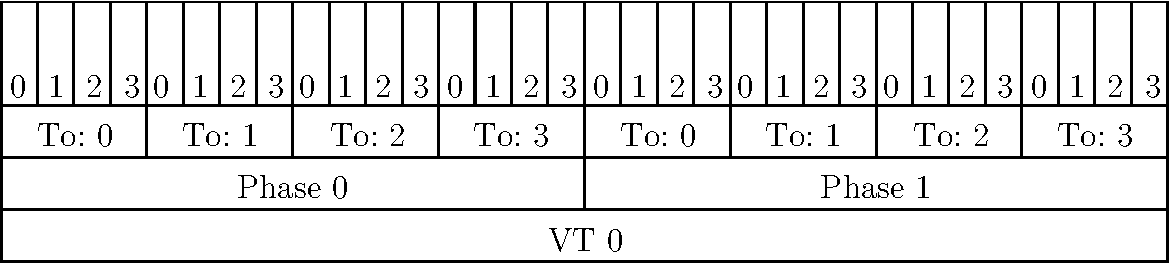
\includegraphics[width=\textwidth]{figures/4d-mapped-memory}
    \caption{A single VT of the 4D array, mapped to 1D memory}
    \label{fig:4d-mapped-memory}
\end{figure}

\subsection{Model and Successor Generation}
\label{section:implementation:successor-generation}

% How are models implemented?
Models are implemented using a data structure that represents a current state.
Each state instance then provides the two operations $\sSuccessor$ and $\sViolates$.
The state instances are stored in the queues.

%% How can states be created on-the-fly on the GPU?
State generation is usually heavily based on branching through \texttt{switch}- and \texttt{if}-conditions.
However, CUDA's SIMT execution model, in which warps of 32 threads operate on same instruction, causes threads to pause when their execution paths diverge.
This means that state generation through branching results in a slower CUDA execution.
As a countermeasure, \citeauthor*{Bartocci2014.GPGPU-Parallel-SPIN} propose to calculate all possible state transitions every time, preserving the SIMT execution and at the same time creating different states in each thread \cite[Algorithm 3]{Bartocci2014.GPGPU-Parallel-SPIN}.
To do so, it makes use of the custom ternary operator described in \cref{alg:branching-free-ternary-operator} that exploits the fact that boolean values evaluate to either zero or one.

\begin{algorithm}
    \caption{Branching-Free Ternary Operator}
    \label{alg:branching-free-ternary-operator}
    \begin{algorithmic}
        \Function{$\branchFreeTernary$}{bool c, int t, int f}
        \State \Return $c \cdot t + (1 - c) \cdot f$
        \EndFunction
    \end{algorithmic}
\end{algorithm}

A key difference of our implementation is that we do not fit a state's variables into a single integer using bit shifts.
Instead, we use regular C++ class data members.
The increased memory demand by regular data members can be neglected, as the queues in which we store state instances are in global memory which is usually gigabytes in size.
Also, the same behavior as in the paper can be achieved using C++ bit field members.

Using our custom ternary, we can re-use DVE models from the BEEM model database\footnote{\url{https://paradise.fi.muni.cz/beem/} (discontinued)}.
DVE is a file format used by the DIVINE 3 model checker.
We translate DVE models into CUDA compatible C++ with the template described in \cref{alg:on-the-fly-state-generation-on-the-gpu}.

% TODO explain the on-the-fly GPU state generation algorithm

\begin{algorithm}
    \caption{On-The-Fly State Generation on the GPU}
    \label{alg:on-the-fly-state-generation-on-the-gpu}
    \begin{algorithmic}
        \LComment{Global variables}
        \State $glob \gets 0$
        \LComment{Process-Local variables use arrays. Here, N is the number of processes}
        \State $state[N] \gets \{0, \dots, 0\}$

        \Statex

        \Function{$\sSuccessor$}{p, ndc, state}
        \LComment{Evaluate all guards before calculating transitions}
        \State $guard_1 \gets state[p] = 0$
        \State $guard_2 \gets state[p] = 1 \land glob \leq 2$
        \State $guard_3 \gets state[p] = 1 \land glob > 2$

        \LComment{Transition from state 0 to 1}
        \State $next.state \gets \branchFreeTernary(guard_1, 1, state.state)$

        \LComment{Transition from state 1 to 1}
        \State $next.glob \gets \branchFreeTernary(guard_2, state.glob + 1, state.glob)$
        \State $next.state \gets \branchFreeTernary(guard_2, 1, next.state)$

        \LComment{Transition from state 1 to 0}
        \State $next.glob \gets \branchFreeTernary(guard_3, 0, next.glob)$
        \State $next.state \gets \branchFreeTernary(guard_3, 0, next.state)$

        \Statex

        \State \Return $next$
        \EndFunction
    \end{algorithmic}
\end{algorithm}

% https://docs.nvidia.com/cuda/cuda-c-programming-guide/index.html#simt-architecture
% https://docs.nvidia.com/cuda/cuda-c-programming-guide/index.html#control-flow-instructions

\subsection{Hash Tables}
\label{section:implementation:hash-tables}

The hash tables provide a data structure in which states are marked as visited.
They are only used on-device within the CUDA kernel and stored in shared memory, resulting in a highly constrained size.
Each VT operates on a single hash table, meaning that all threads in a block share one hash table.
For memory efficiency, we use bitstate hashing \cite{DeFrancisco2020.Grapple}.
Our hash tables can store $2^{18}=\num{262144}$ states, taking up \num{32768} bytes of shared memory.

% How does bitstate hashing work?
In bitstate hashing, a single bit represents whether a state is visited.
Per clock cycle, CUDA can transmit 32 bit of shared memory, which is stored in 32-bit words.
Resulting from this, we use a bucket size of 32 bit.
The bit representing whether a state is visited is then computed using \cref{alg:bitstate-hashing}.

% How can we control collisions?
The hash function's goal is to map random data with unknown distribution onto a nearly uniform distribution, so each bucket of the hash table is used equally likely.
In our implementation, hashing is done using the Jenkins Hash function \cite{JenkinsHash}.
The MurmurHash3 \cite{MurmurHash3}, which is used by our HyperLogLog, yields similar results.

Hash collisions resulting in false-positives are intended, as explained in \cref{section:theory:hash-table}.
To achieve that in every VT different states cause a collision, each is including a different seed into the hash.
The rate of collisions can then be controlled by the hash table's size.

\begin{algorithm}
    \caption{Bitstate hashing}
    \label{alg:bitstate-hashing}
    \begin{algorithmic}
        \LComment{Initialize hash table buckets. Here, $N$ is the hash table size}
        \State $table[(1 << N - 5)] \gets \{0, \dots, 0\}$

        \Statex

        \Function{$\markVisited$}{table, state}
        \State $hash \gets \makeHash(state, seed) \bitwiseAnd (1 << N) - 1$

        \LComment{First 5 bits ($2^5=32$) are the index within the bucket}
        \State $elem \gets hash >> (N - 5)$

        \LComment{Last $N-5$ bits are the bucket index}
        \State $bucket \gets hash \bitwiseAnd (1 << N - 5) - 1$

        \LComment{Retrieve current state}
        \State $isVisited \gets table[bucket] \bitwiseAnd (1 << elem) \neq 0$

        \LComment{Update hash bucket}
        \State $table[bucket] \gets table[bucket] \bitwiseOr (1 << elem)$

        \Statex

        \State \Return $isVisited$
        \EndFunction
    \end{algorithmic}
\end{algorithm}

\subsection{HyperLogLog++}

The HyperLogLog (HLL) provides an algorithm for distributed counting of distinct elements, as described in \cref{section:theory:counting-unique-states-visited}.
In our implementation, the grid of VTs of each run is operating on a single HLL that is stored in global memory.
Visited states are added to the HLL only on-device.
The host collects the HLLs after the kernels have finished, merge them into one big HLL and does the estimation of unique states visited.
Merging and estimating the amount of unique states visited is done only on the host.

\section{Usage}
\label{section:implementation:usage}

To verify a model using our model checker, a user has to complete the following steps:

\begin{enumerate}
    \item Describe their model in a C++ class using \cref{alg:on-the-fly-state-generation-on-the-gpu}
    \item Compile our model checker including their model
    \item Execute the single output binary.
          On execution, the user may set the PRNG seed and number of runs using command-line options.
          The number of runs needed to achieve a certain state space coverage needs to be evaluated experimentally.
    \item Interpret the CSV output
\end{enumerate}

\chapter{Evaluation}
\label{chapter:evaluation}

% This chapter presents empirical experimental results of our implementation.
This chapter presents our series of empirical experiments conducted on our implementation.
It starts with experiments on the correctness of our implementation and a comparison with the Grapple paper's results in \cref{section:evaluation:correctness-comparison-with-paper}.
We then continue with a series of experiments that compare the Waypoints model, which is known to be high-connectivity, with three low-connectivity models in \cref{section:evaluation:low-connectivity-model-evaluation}.

All experiments are performed on an NVIDIA GeForce RTX 2080 Ti GPU, AMD Ryzen Threadripper 2990WX CPU and \SI{128}{\giga\byte} main memory using Ubuntu 20.04.2 LTS.
All values related to state space coverage are estimated using a HLL with $2^{14}$ registers and thus prone to an error, as explained in \cref{section:theory:counting-unique-states-visited}.

\section{Correctness and Comparison with the Paper}
\label{section:evaluation:correctness-comparison-with-paper}

We start the evaluation with whether our implementation reaches the same number of discovered waypoints in relation to the amount of executed VTs as presented in the Grapple paper.
We would expect both implementation to behave similarly, discovering at least 80 waypoints in \num{20000} VTs and all 100 waypoints in about \num{100000} VTs, as shown in \cref{fig:evaluation:EXP-00:1}.
However, that is clearly not the case, as presented in \cref{fig:evaluation:EXP-00:2}.
Our implementation found significantly fewer waypoints, even though the amount of VTs was 2.5x larger.

To further investigate differences between the implementations, we conducted additional experiments.

\begin{figure}
    \begin{subfigure}[b]{.5\textwidth}
        \centering
        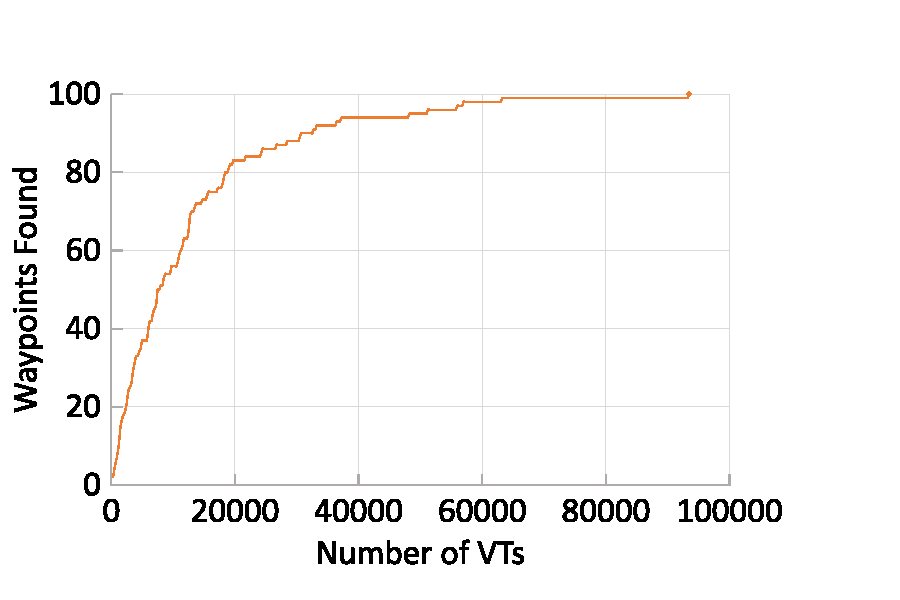
\includegraphics[width=\textwidth]{../evaluation/assets/EXP-00-grapple-paper-waypoints.pdf}
        \subcaption{Results from the paper}
        \label{fig:evaluation:EXP-00:1}
    \end{subfigure}
    \begin{subfigure}[b]{.5\textwidth}
        \centering
        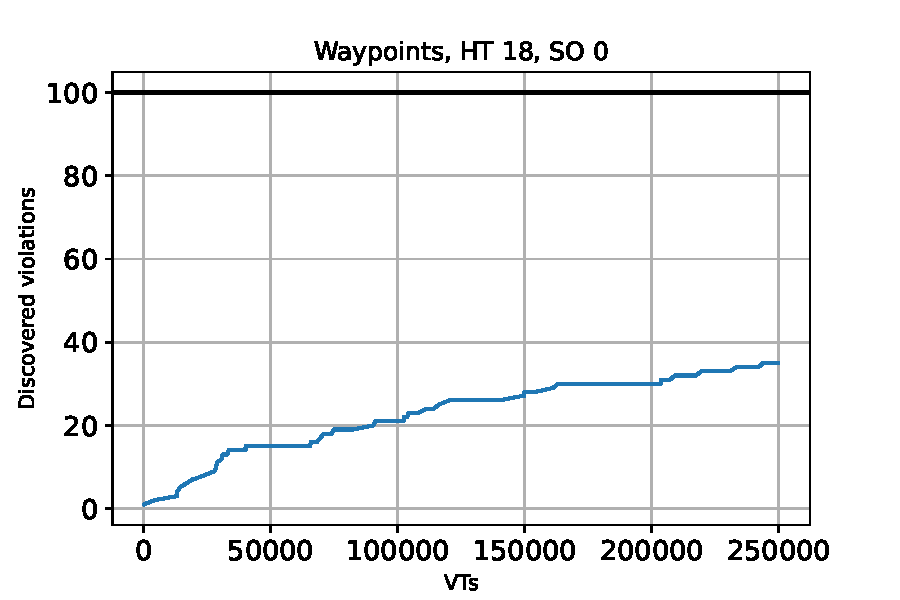
\includegraphics[width=\textwidth]{../evaluation/output-assets/EXP-00-comparison-with-paper.pdf}
        \subcaption{Results of our implementation}
        \label{fig:evaluation:EXP-00:2}
    \end{subfigure}
    \caption{Waypoints model, comparison between reference and our implementation}
    \label{fig:evaluation:EXP-00}
\end{figure}

\subsection{Comparison of Waypoints and HLL as Estimators of State Space Coverage}

As explained in \cref{section:theory:waypoints-model}, counting waypoints is a method for estimating the achieved state space coverage.
To make sure that the discovered waypoints of our implementation correctly indicate the state space coverage, we compared them to the state space coverage estimation of the HyperLogLog introduced in \cref{section:theory:counting-unique-states-visited}.
We would expect both estimators to show similar results.
For example, when 20 waypoints are discovered, the HyperLogLog estimation should show about \SI{20}{\percent} state space coverage.

\cref{fig:evaluation:EXP-01} presents results for both estimators.
Clearly, both resemble each other closely.
Thus, we assume them to work correct.
This also confirmed the results from our first experiment, underlining our implementation's deficient state space exploration.

\begin{figure}[h]
    \begin{subfigure}[b]{.5\textwidth}
        \centering
        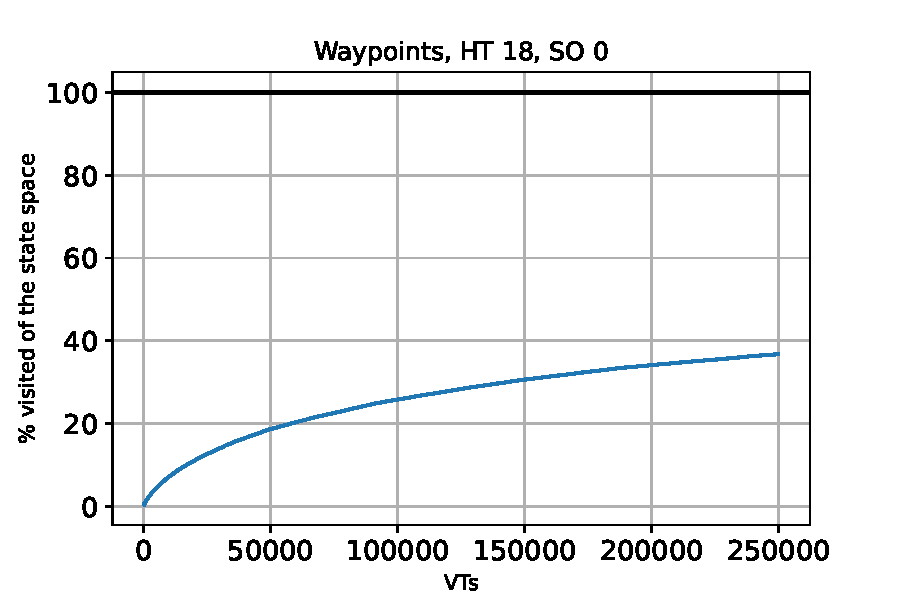
\includegraphics[width=\textwidth]{../evaluation/output-assets/EXP-01-comparison-waypoints-hll-1.pdf}
        \subcaption{HLL state space coverage estimation}
        \label{fig:evaluation:EXP-01:1}
    \end{subfigure}
    \begin{subfigure}[b]{.5\textwidth}
        \centering
        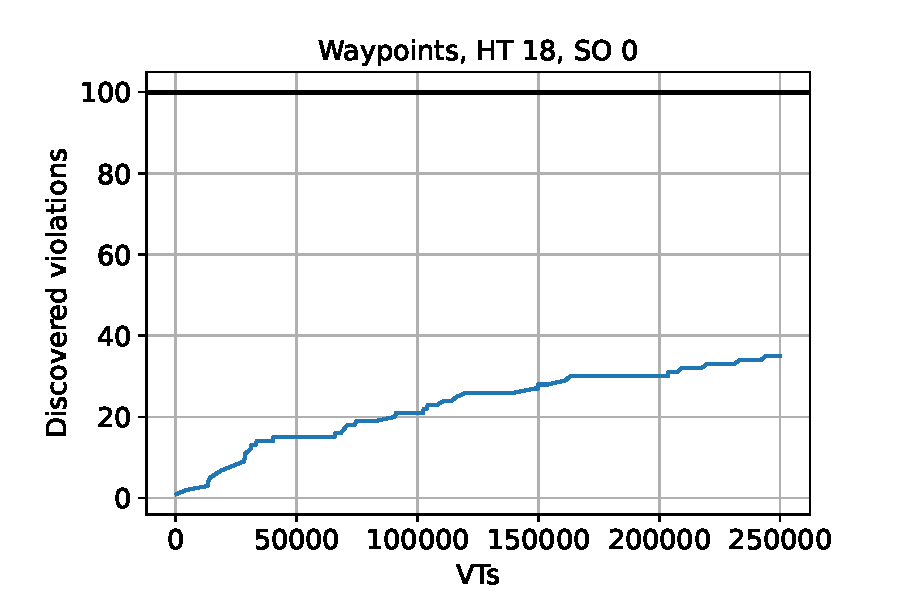
\includegraphics[width=\textwidth]{../evaluation/output-assets/EXP-01-comparison-waypoints-hll-2.pdf}
        \subcaption{Waypoints state space coverage estimation}
        \label{fig:evaluation:EXP-01:2}
    \end{subfigure}
    \caption{Comparison between Waypoints and HyperLogLog state space coverage estimation}
    \label{fig:evaluation:EXP-01}
\end{figure}

\subsection{Impact of Hash Table Size and Sequential VT Execution}

Both implementations share a queue size of $32 \times 32 \times 4$.
Beside of that, we identified two key differences of our implementation:

\begin{itemize}
    \item Our hash tables are \SI{33}{\percent} smaller than in the paper.
          This is due to our bit shift implementation presented in \cref{section:implementation:hash-tables} which cannot address the full \SI{48}{\kibi\byte} of shared memory.
    \item We batch VTs in a CUDA kernel, each executing 250 at once.
          In the paper, there seems to be only a single VT per CUDA kernel.
\end{itemize}

To find out whether increasing the hash table size to full \SI{48}{\kibi\byte} increases waypoint discovery such that it is similar to the results from the Grapple paper, we experimentally changed our implementation's addressing.
As the hash table capacity should significantly affect the state space coverage of each VT, we would expect results close to those from the paper.
For each experiment, we executed 80 runs à 250 VTs (= \num{20000} VTs in total).
Results are shown in \cref{table:EXP-02}.

The larger hash table yielded 2.1x as much state space coverage at only 1.45x as many total states visited.
Thus, a larger hash table seems beneficial on this particular model.

However, in the paper, a Grapple swarm verification with \num{392800} hash table slots per VT discovered 85 waypoints in \num{20000} VTs, equalling \SI{85}{\percent} state space coverage, which is about 3.7x as much as our large-size hash table implementation.
Resulting from this, the large-size hash table is still far from reproducing the paper's results.

\begin{table}
    \caption{Exploration of the waypoints model using different hash table capacities in 80 runs à 250 VTs}
    \label{table:EXP-02}
    \centering
    \begin{tabular}{l l l l}
        \toprule
        HT Capacity  & State Space Coverage & Total States Visited \\
        \midrule
        \num{262144} & \SI{11.04}{\percent} & \num{63568607}       \\
        \num{393056} & \SI{23.14}{\percent} & \num{91937680}       \\
        \bottomrule
    \end{tabular}
\end{table}

In the paper, supposedly one VT is executed per \emph{grid}, resulting in one CUDA kernel per VT.
To compare our parallelization of VTs in a single CUDA kernel with the sequential execution of multiple kernels, we switched the compiled number of VTs and the executed runs.
We would expect both variants to create similar results.
Furthermore, we would expect a shorter execution time of the parallel execution as it only needs a single kernel setup.
Results for both variants are shown in \cref{table:EXP-03}.
The state space coverage and total visited states of both experiments are highly similar.
The execution time of parallel execution was more than 35x faster.
Concluding this, the experiment showed that batch execution of VTs highly speeds up execution time at equal results.

\begin{table}
    \caption{Parallel and sequential exploration of the waypoints model}
    \label{table:EXP-03}
    \centering
    \begin{tabular}{l l l l S}
        \toprule
        {VTs per Kernel} & {Runs} & {State Space Coverage} & {Total States Visited} & {Execution Time}     \\
        \midrule
        1                & 250    & \SI{0.456}{\percent}   & \num{63568343}         & \SI{26.691}{\second} \\
        250              & 1      & \SI{0.450}{\percent}   & \num{63568498}         & \SI{0.754}{\second}  \\
        \bottomrule
    \end{tabular}
\end{table}

The last two experiments showed that there seems to be a lack in our implementation beside the hash table capacity, queue size and execution order.

\subsection{Increasing State Space Coverage using Start Overs}
\label{section:evaluation:start-overs}

We suspect that part of the bad exploration performance is that each VT can only reach as deep into the state space as its hash table can find unvisited states.
As a countermeasure, we introduced the start over strategy in \cref{section:theory:start-overs}.

The next experiment evaluates whether start overs actually increase the growth of state space coverage and thus the model checking performance.
By reaching deeper states, we would expect to discover more violations and thus a faster growing state space coverage.
To do so, we compared \num{1000} exploration runs of the waypoints model with an arbitrary, much lower hash table capacity of $2^{14}=\num{16384}$ slots and 15 start overs with the default configuration of $2^{18}=\num{262144}$ hash table slots and 0 start overs.
We chose 15 start overs to mitigate the smaller hash table, which is $\frac{1}{16}$ the size, resulting in 16 total searches, including the initial search.
Results for both explorations are presented in \cref{fig:evaluation:EXP-04:1}.
With start overs, the exploration took \SI{243}{\second}.
Without, it took \SI{442}{\second}.

As the number of total visited states by a VT varies between the two explorations due to for example different hash collisions, we also compared the cumulated number of total visited states of both explorations in \cref{fig:evaluation:EXP-04:2}.

Clearly, the start over strategy resulted in a significant increase of discovered violations on a similar number of visited states and VTs.
Also, the execution time of the start over strategy was 1.82x faster.
We conclude that start overs create a significant performance increase on the waypoints model.

\begin{figure}
    \begin{subfigure}[b]{.5\textwidth}
        \centering
        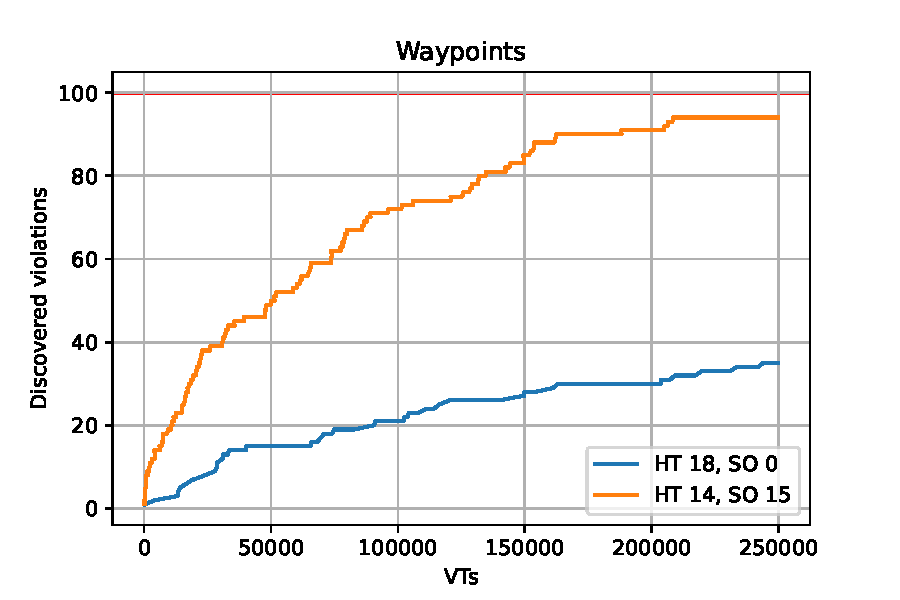
\includegraphics[width=\textwidth]{../evaluation/output-assets/EXP-04-start-overs-1.pdf}
        \subcaption{Comparison of discovered waypoints}
        \label{fig:evaluation:EXP-04:1}
    \end{subfigure}
    \begin{subfigure}[b]{.5\textwidth}
        \centering
        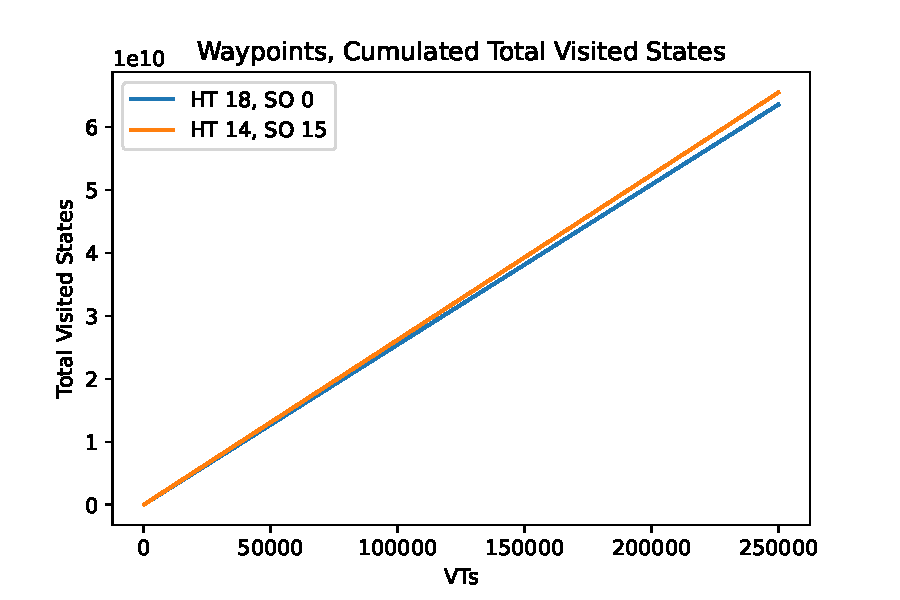
\includegraphics[width=\textwidth]{../evaluation/output-assets/EXP-04-start-overs-3.pdf}
        \subcaption{Comparison of total visited states}
        \label{fig:evaluation:EXP-04:2}
    \end{subfigure}
    \caption{State space exploration with start overs}
    \label{fig:evaluation:EXP-04}
\end{figure}

% TODO section summary

\section{Low-Connectivity Model Evaluation}
\label{section:evaluation:low-connectivity-model-evaluation}

% TODO link to low-connectivity definition and introduction
In this section, we try to make key differences of low-connectivity state space exploration tangible.
The paper suspects three models of being low-connectivity:

\begin{itemize}
    \item Dining philosophers problem
    \item Anderson queue lock mutual exclusion algorithm
    \item Peterson mutual exclusion protocol
\end{itemize}

\subsection{Dining Philosophers Problem with Different Numbers of Processes}

The paper suggests that a state space size surpassing the hash table capacity significantly slows down the state space exploration, resulting in a higher number of VTs needed to achieve $>\SI{99}{\percent}$ state space coverage.
To find out how much the state space size affects the exploration performance, we compared three variants with \numlist{11;12;13} processes of the dining philosophers problem.
Using our default hash table capacity of $2^{18}$ slots, we would expect a slow-down starting with 12 processes, as fewer processes have a state space size smaller than the hash table capacity.
As presented in \cref{table:EXP-10}, exploring DP-13 took 213x the VTs as for DP-11, even though it is only 9x its state space size.
This confirmed our hypothesis of a significant slow-down for this particular model.

\begin{table}
    \caption{Exploration of the dining philosophers problem with \numlist{11;12;13} processes}
    \label{table:EXP-10}
    \centering
    \begin{tabular}{l l l l}
        \toprule
        Model & State Space Size & Hash Table Utilization & \# of VTs to explore                  \\
        \midrule
        DP-11 & \num{177146}     & ~\SI{68}{\percent}     & \SI{100}{\percent} in 250 VTs         \\
        DP-12 & \num{531440}     & ~\SI{203}{\percent}    & \SI{100}{\percent} in 250 VTs         \\
        DP-13 & \num{1594322}    & ~\SI{608}{\percent}    & \SI{100}{\percent} in \num{53250} VTs \\
        \bottomrule
    \end{tabular}
\end{table}

\subsection{Comparison of Unique States Visited, Total States Visited and State Space Coverage}

In the paper, the models yielded very different results concerning the unique and total states visited.
Thus, the next experiment compares these performance indicators for our set of models on a fixed amount of \num{125000} VTs.
We would expect clear differentiation between the models and eventually a clear distinction between high- and low-connectivity.
Our results are displayed in \cref{table:EXP-12}.
Clearly, the waypoints model achieved the highest number of total states visited.
We further observed an interesting property by taking the unique states visited in relation to the total states visited, presented in the \emph{Rate} column:
All three low-connectivity models achieved a rate $< \SI{0.1}{\percent}$.
In conclusion, the performance deficiency of the three presented low-connectivity models can be observed through unique states visited and total states visited.

\begin{table}
    \caption{Exploration of low-connectivity models, each after \num{125000} VTs}
    \label{table:EXP-12}
    \centering
    \begin{tabular}{l l l l l}
        \toprule
        Model      & Unique States Visited & Total States Visited & Rate                 \\
        \midrule
        Anderson 3 & \num{1.22779e+06}     & \num{15477969183}    & \SI{0.008}{\percent} \\
        Peterson 5 & \num{4.08578e+06}     & \num{24670432336}    & \SI{0.017}{\percent} \\
        DP 15      & \num{1.38213e+07}     & \num{30436723433}    & \SI{0.045}{\percent} \\\addlinespace
        Waypoints  & \num{1.21759e+09}     & \num{35725590331}    & \SI{3.408}{\percent} \\
        \bottomrule
    \end{tabular}
\end{table}

\subsection{BFS Frontiers of Low-Connectivity Models}

The algorithm introduced in \cref{section:theory:grapple-model-checker} is operating in alternating phases that produce so-called \emph{frontiers}.
Each frontier is an intermediate state of the BFS, representing the deepest states found until now.
A new frontier is built by checking whether generated successors were visited before.
For this experiment, we call already visited states \emph{failed} and states added to the new frontier \emph{visited}.
To find out whether different models affect the BFS frontiers in terms of visited and failed states, we executed a single VT and counted visited and failed states for each frontier generated.

In Grapple, each BFS starts with a single initial state.
As of this, we would expect the number of visited states to quickly build up until the number of failed states takes over due to the hash tables filling up.

\begin{samepage}
    For visualization of BFS frontiers, we provide two different methods:

    \begin{itemize}
        \item Plotting the absolute number of visited and failed states.
        \item Plotting visited and failed states in relation to each other, both adding up to \SI{100}{\percent}.
    \end{itemize}
\end{samepage}

\cref{fig:evaluation:EXP-11-1} presents both visualizations for the waypoints model.
As expected and shown in the absolute representation on the left, the amount of visited states quickly built up and then decayed until the BFS terminated.
We observed similar behavior in the relative representation shown on the right:
The search started with only visited states, which decayed quickly as the failed states took over until the search terminated.
The relative representation contained an interesting anomaly in the build up phase between BFS round 0 and 5, where in one round, the relative amount of visited states suddenly grew again.

Visualizations of low-connectivity models are presented in \cref{fig:evaluation:EXP-11-2}.
The dining philosophers and Peterson model both showed a behavior similar to the waypoints model.
There is one characteristic only shared by the low-connectivity models:
In their relative representations, they all had two spikes of visited states right before their search terminated.
We suspect them to be a characteristic of low-connectivity models, but this assumption needs additional research.

The Anderson model in contrast showed completely unexpected behavior:
In the absolute representation on the left, neither a constant maximum of visited and failed states, nor the typical build-up-then-decay-process could be observed.
Instead, there is a notch between BFS round 50 and 100 where the amount of both visited and failed states over multiple BFS rounds went down, then built up again.
We suspect that this notch could be a sign for a bottleneck, but this assumption also needs additional research.
Furthermore, the relative representation on the right showed a near constant amount of around \SI{40}{\percent} visited states per BFS round, with two salient spikes on the end before out of a sudden the search terminated.

% TODO conclusion of this experiment?
% TODO also interesting: the number of BFS rounds an number of states highly differs between models

\begin{figure}
    \begin{subfigure}[b]{.5\textwidth}
        \centering
        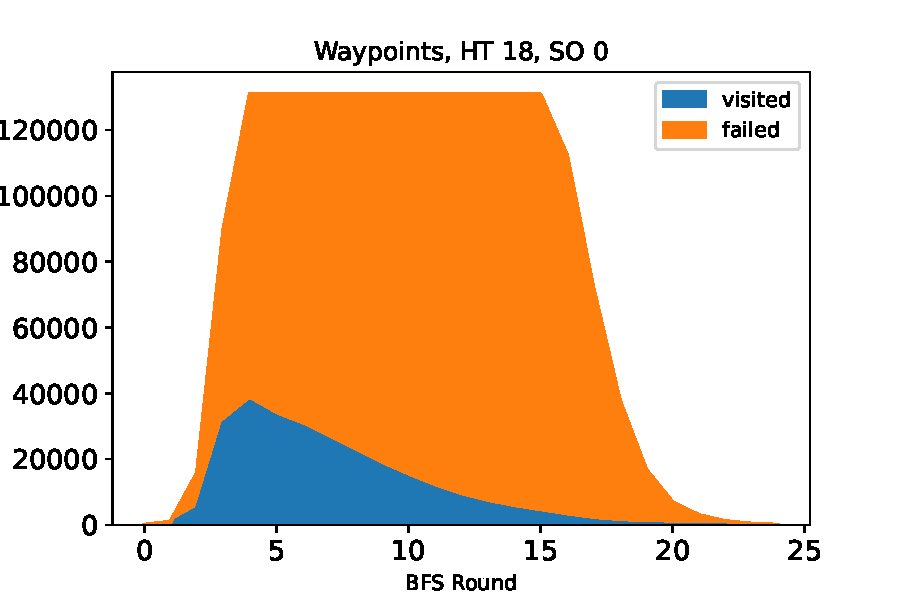
\includegraphics[width=\textwidth]{../evaluation/output-assets/EXP-11-bfs-frontiers-1.pdf}
        \label{fig:evaluation:EXP-11:1}
    \end{subfigure}
    \begin{subfigure}[b]{.5\textwidth}
        \centering
        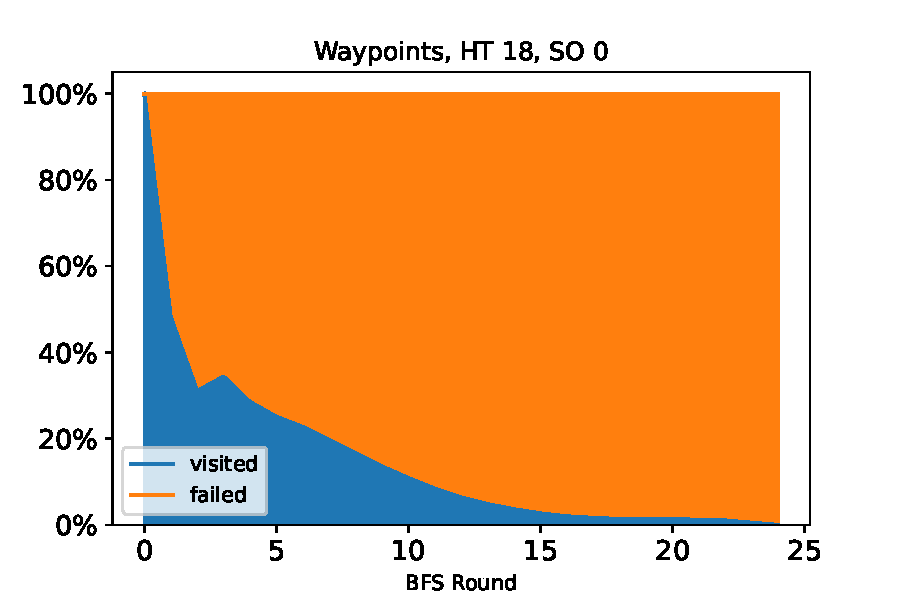
\includegraphics[width=\textwidth]{../evaluation/output-assets/EXP-11-bfs-frontiers-5.pdf}
        \label{fig:evaluation:EXP-11:5}
    \end{subfigure}
    \caption{BFS frontier visualization of the waypoints model}
    \label{fig:evaluation:EXP-11-1}
\end{figure}

\begin{figure}[p]
    \begin{subfigure}[b]{.5\textwidth}
        \centering
        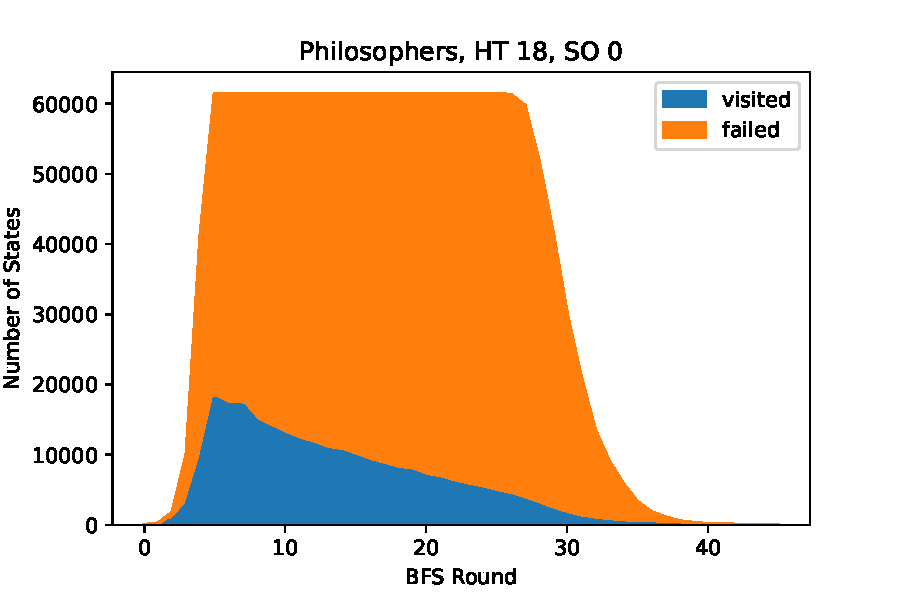
\includegraphics[width=\textwidth]{../evaluation/output-assets/EXP-11-bfs-frontiers-2.pdf}
        \label{fig:evaluation:EXP-11:2}
    \end{subfigure}
    \begin{subfigure}[b]{.5\textwidth}
        \centering
        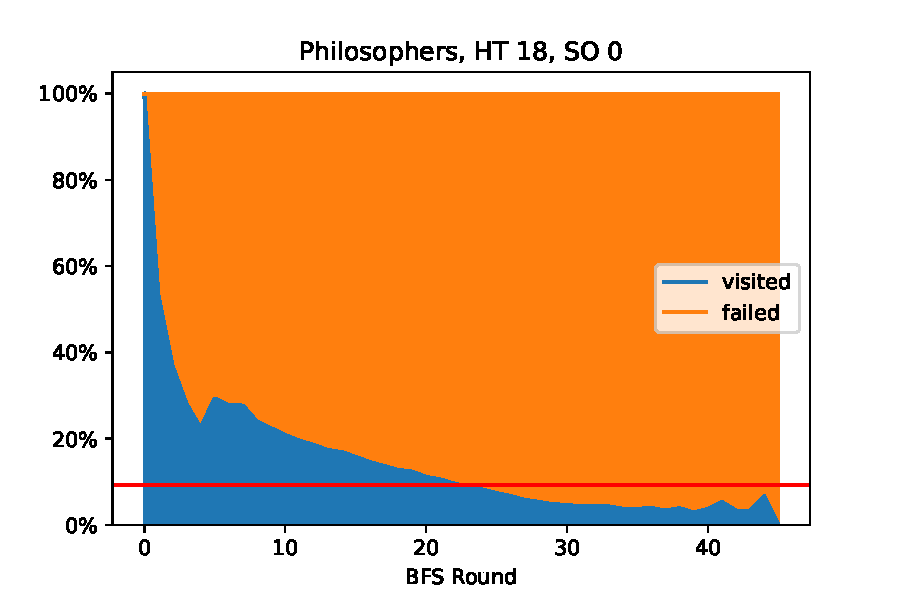
\includegraphics[width=\textwidth]{../evaluation/output-assets/EXP-11-bfs-frontiers-6.pdf}
        \label{fig:evaluation:EXP-11:6}
    \end{subfigure}

    \begin{subfigure}[b]{.5\textwidth}
        \centering
        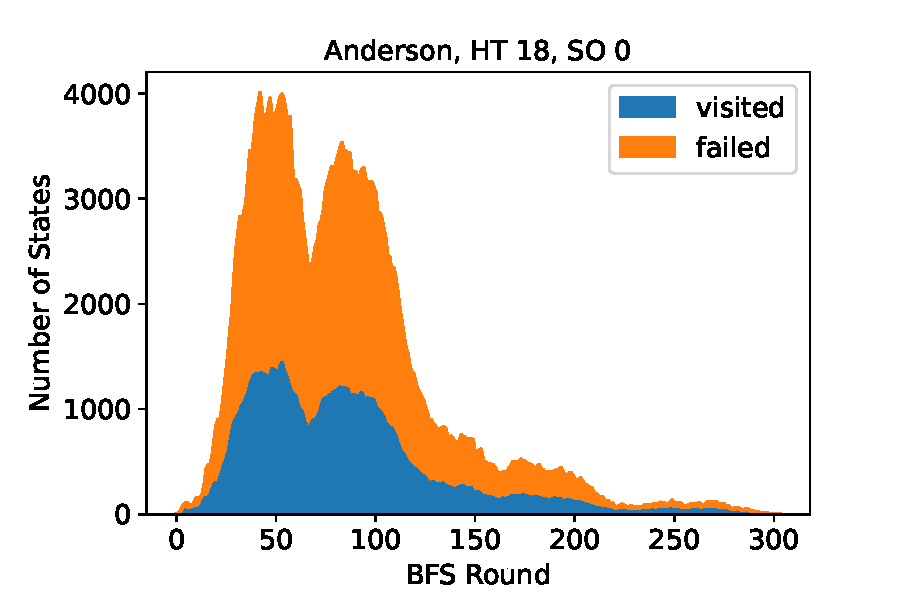
\includegraphics[width=\textwidth]{../evaluation/output-assets/EXP-11-bfs-frontiers-3.pdf}
        \label{fig:evaluation:EXP-11:3}
    \end{subfigure}
    \begin{subfigure}[b]{.5\textwidth}
        \centering
        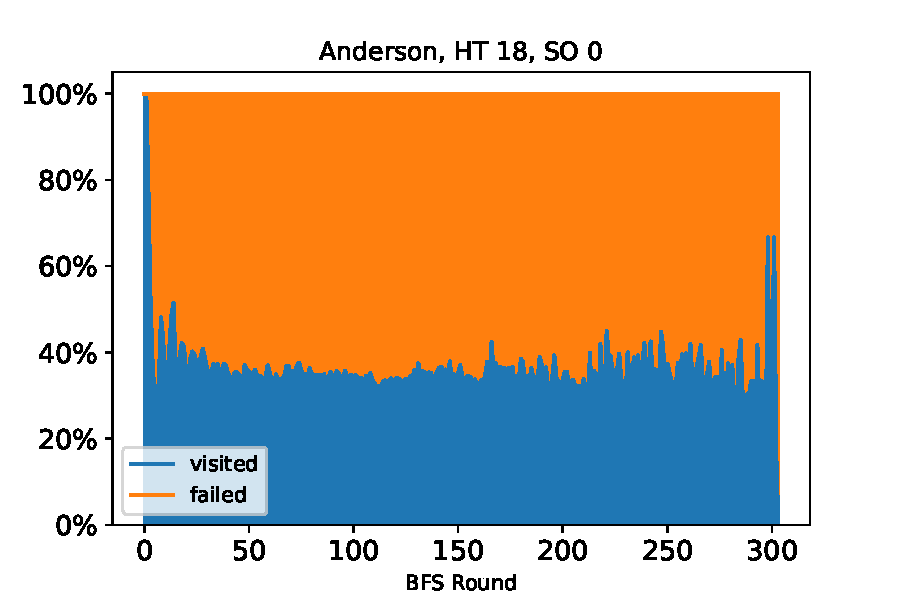
\includegraphics[width=\textwidth]{../evaluation/output-assets/EXP-11-bfs-frontiers-7.pdf}
        \label{fig:evaluation:EXP-11:7}
    \end{subfigure}

    \begin{subfigure}[b]{.5\textwidth}
        \centering
        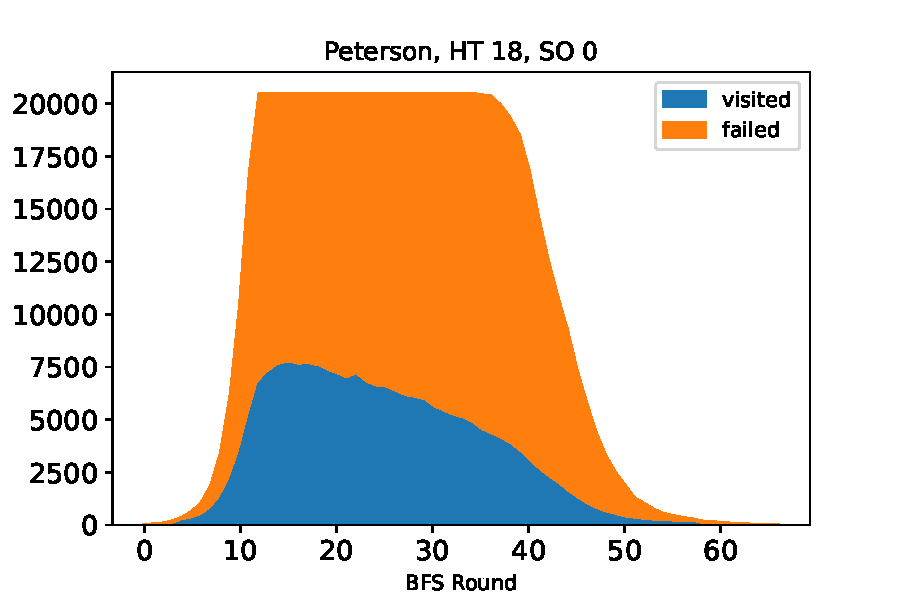
\includegraphics[width=\textwidth]{../evaluation/output-assets/EXP-11-bfs-frontiers-4.pdf}
        \label{fig:evaluation:EXP-11:4}
    \end{subfigure}
    \begin{subfigure}[b]{.5\textwidth}
        \centering
        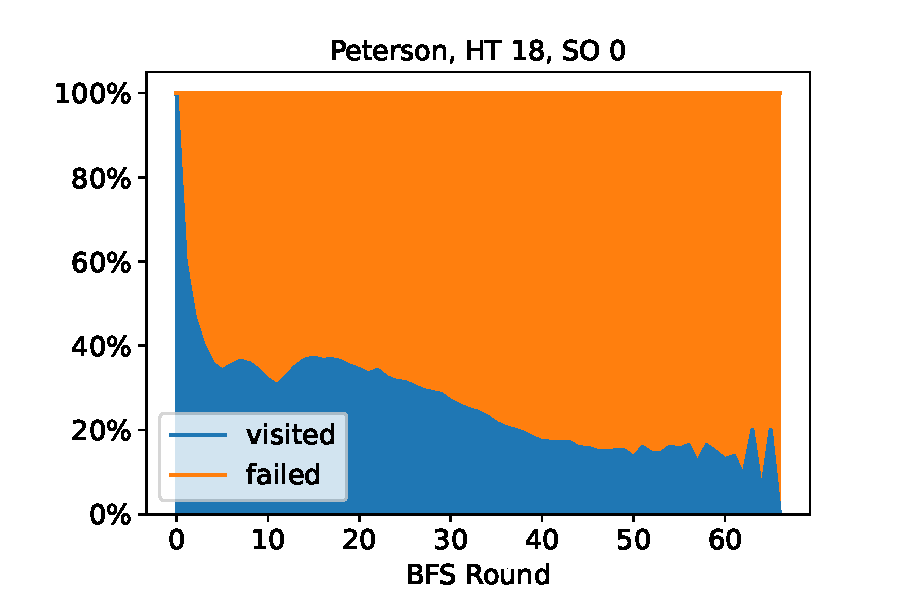
\includegraphics[width=\textwidth]{../evaluation/output-assets/EXP-11-bfs-frontiers-8.pdf}
        \label{fig:evaluation:EXP-11:8}
    \end{subfigure}

    \caption{BFS frontier visualization of low-connectivity models}
    \label{fig:evaluation:EXP-11-2}
\end{figure}

% \FloatBarrier

\subsection{Start Over Strategy on Low-Connectivity Models}

Our last experiment evaluates whether the start over strategy yields the same performance benefit shown in \cref{section:evaluation:start-overs} on low-connectivity models.
For each of our three low-connectivity models, we conducted two explorations of 500 runs à 250 VTs.
One with $2^{18}$ hash table slots and 0 start overs, the other one with $2^{14}$ hash table slots and 15 start overs (same configuration as in \cref{section:evaluation:start-overs}).
As the paper has shown that increasing the search depth can increase coverage on low-connectivity models, we would expect our start over strategy to do so as well.

Plots of the results are presented in \cref{fig:evaluation:EXP-13}.
The most interesting observation is that on the Anderson model, start overs significantly worsened the state space coverage in relation to the executed VTs.
Beyond that, the dining philosophers and Peterson model fulfilled our expectation with a slightly improved state space coverage.
Looking at the execution time, start overs sped up the execution time on all three models:
The dining philosophers model executed 1.15x faster, the Anderson model 1.82x faster and the Peterson model 1.2x faster.

In conclusion, the experiment has shown that start overs can actually improve exploration performance in terms of state space coverage and execution time on the presented models, with the Anderson model being an exception that needs further investigation.

\begin{figure}
    \begin{subfigure}[b]{.5\textwidth}
        \centering
        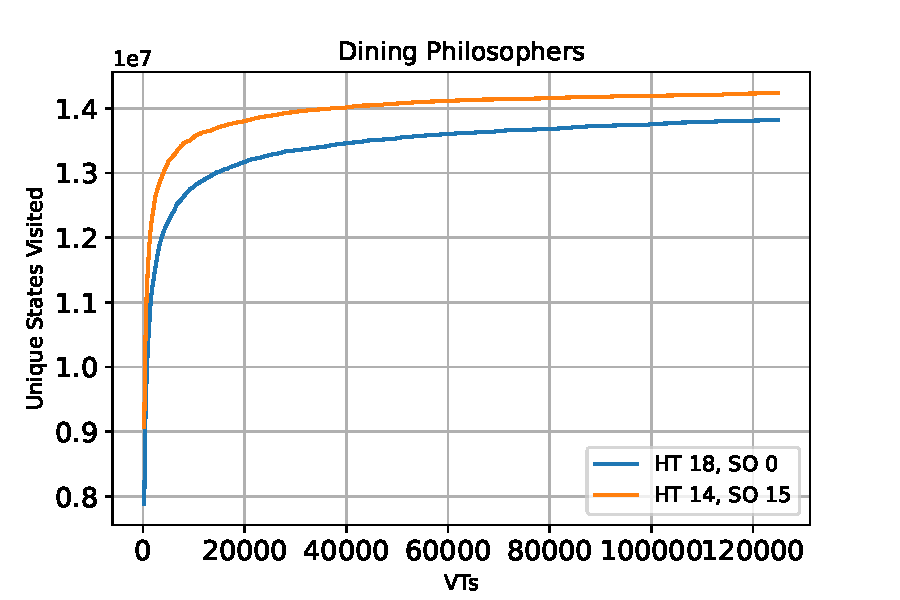
\includegraphics[width=\textwidth]{../evaluation/output-assets/EXP-13-start-overs-low-connectivity-1.pdf}
        \label{fig:evaluation:EXP-13:1}
    \end{subfigure}
    \begin{subfigure}[b]{.5\textwidth}
        \centering
        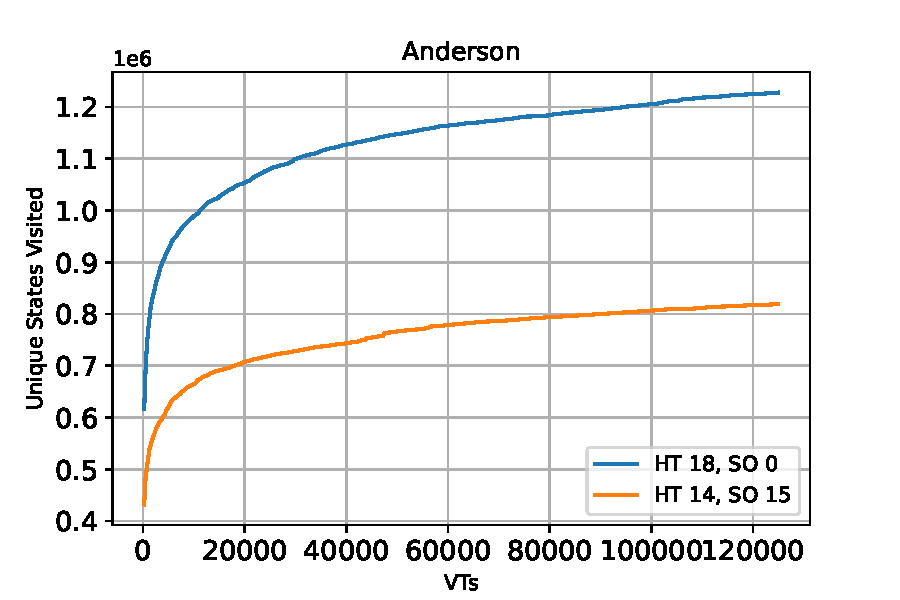
\includegraphics[width=\textwidth]{../evaluation/output-assets/EXP-13-start-overs-low-connectivity-2.pdf}
        \label{fig:evaluation:EXP-13:2}
    \end{subfigure}
    \begin{subfigure}[b]{\textwidth}
        \centering
        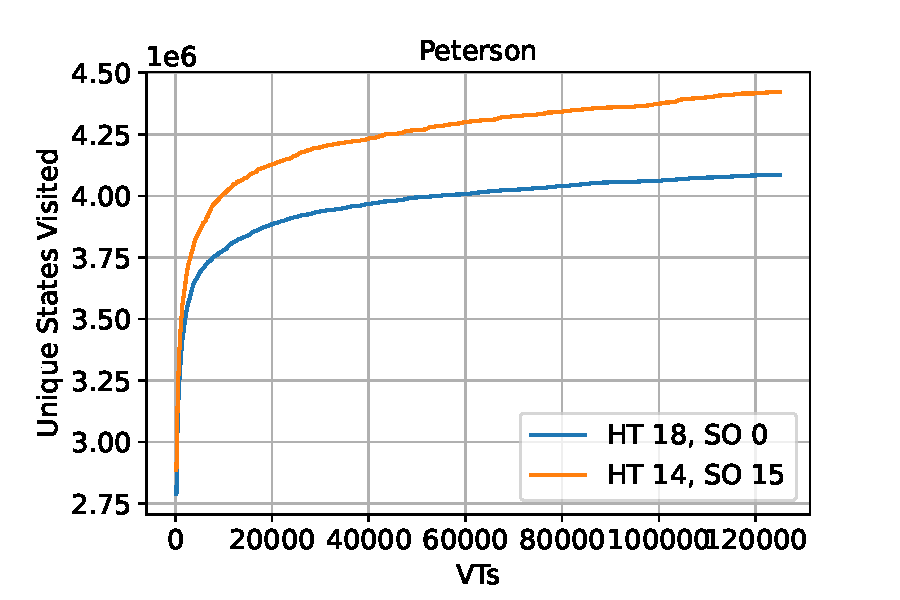
\includegraphics[width=.5\textwidth]{../evaluation/output-assets/EXP-13-start-overs-low-connectivity-3.pdf}
        \label{fig:evaluation:EXP-13:3}
    \end{subfigure}
    \caption{Start over strategy on low-connectivity models}
    \label{fig:evaluation:EXP-13}
\end{figure}

\chapter{Conclusion}
\label{chapter:conclusion}

\section{Future Work}

\begin{itemize}
    \item Estimate state space size for models of unknown size
    \item Automatically determine the optimal number of start overs
    \item Implement usage of multiple GPU devices through CUDA streaming API
    \item Analyze State Space Diversification, i.e. "how good is a partition?"
\end{itemize}

\section{Discussion}

\begin{itemize}
    \item As in the evaluation: The Anderson model draws special interest: Its BFS frontiers show a unique behavior and using the start over strategy, it performs contrary to all other models.
\end{itemize}

% \appendix

% \chapter{Listings}

\backmatter

\printbibliography[heading=bibintoc]

\end{document}
